%\documentclass[titlepage]{extarticle}
\documentclass[9pt, titlepage]{extarticle}
\usepackage{appendix}
\usepackage{wrapfig}
\usepackage[T1]{fontenc}
\usepackage{lipsum}
\usepackage[utf8]{inputenc} % allows UTF-8, support special characters
\usepackage[UKenglish]{babel} % use UK English hyphenation rules
\usepackage{csquotes} % recommended by babel, better quotes
%\usepackage[a4paper, margin=2.5cm]{geometry} % smaller margins, see below
\usepackage[a4paper, margin=2.15cm]{geometry} % smaller margins, see below
\usepackage{titlesec}
\usepackage{tabularx}
\usepackage{enumitem}
\usepackage{subcaption}
\usepackage{float}
\usepackage{tabto}
\usepackage[style=numeric, sorting=none]{biblatex}
\usepackage{graphicx} % allows images
\usepackage{hyperref} % automatically links references within the document
\renewcommand*{\bibfont}{\small}
\setlength\bibitemsep{1mm}
\usepackage{subfig}

\addbibresource{ref.bib} % links bibiography file
%\usepackage{nimbusmono}
%\renewcommand*{\ttdefault}{nimbusmono}

\titleclass{\subsubsubsection}{straight}[\subsection]
\newcounter{subsubsubsection}[subsubsection]
\renewcommand\thesubsubsubsection{\thesubsubsection.\arabic{subsubsubsection}}
\titleformat{\subsubsubsection}
  {\normalfont\normalsize\bfseries}{\thesubsubsubsection}{1em}{}
\titlespacing*{\subsubsubsection}
{0pt}{3.25ex plus 1ex minus .2ex}{1.5ex plus .2ex}
\makeatletter
\def\toclevel@subsubsubsection{4}
\def\l@subsubsubsection{\@dottedtocline{4}{7em}{4em}}
\makeatother
\setcounter{secnumdepth}{4}
\setcounter{tocdepth}{4}
\setlength{\parindent}{0pt}

\title{Final Report}
\author{
\textbf{Group 32} \\\\
Module Organiser: Dr. James Archbold \\
Tutor: Mahshid Mehr Nezhad \\\\
Alexander Price \\
Thomas Cowley \\
George Denny \\
Yang Tang \\
Moustafa Eladawy
}
\date{March 2021}

\begin{document}

\Large{
\emph{Final Report, Group 32}
\hfill
March 2021}
\normalsize{}

% \Large{
% \emph{Design and Planning Document, Group 32}
% \hfill
% February 2021}
% \normalsize{}

\section{Introduction}
This document details the final report for a project to develop a product that can accept feedback during live events, and analyse it in real time, presenting useful information to event hosts. It discusses the final product and the development process.

\section{Project Record}

This section details the events of product development, documenting them using the Scrum sprint cycles outlined in the design and planning document \cite{design-and-planning}. It breaks each cycle into two records. The first describes the strict occurrences of development. The second details the issues encountered and mitigation strategies created in response. This second section also discusses and evaluates the evolution of the projects management and methodology.

\subsection{First Sprint Cycle: Feb 1 - Feb 7}

\subsubsection{Development}
% PLANNED: Init and Front-end

The plan for the first sprint cycle was to initialise the project and develop the front-end. Initialising the project involved generating a project structure and repository, integrating Maven with the project and adding dependencies, and setting up a database server instance capable of communicating with the project.\\

Project initialisation was completed as planned, however it became apparent that the method of interaction between the database and the Spark Java system back-end \cite{web:spark} was not considered in the design. As a result, additional unplanned labour was required to evolve the design and implement a solution, using Docker \cite{docker}.\\

It was also discovered that the React framework \cite{web:react} was unsuitable for the project. Thus, the design again had to be amended and a new solution implemented, incurring additional labour costs. The HTML5 stack (HTML, CSS, JS) was used instead, in union with Apache Velocity. This is fully detailed in the Front-End Technologies section of the Requirements and Design evolution section evolution. Design evolution was completed - however, front-end development based on the evolved design was not started.\\

Communication channels were refocused around development, and documentation frameworks were created to assist and facilitate coordination and organisation. This was done through the use of a Discord \cite{discord} - a VoIP, instant messaging and digital distribution platform - as well as HackMD, \cite{hackmd} a shared markdown environment. Additionally, developers were provided with framework documentation to assist in component development.\\

Requirement 1.1.D was also evolved - this is detailed in the Requirements and Design Evolution section. The development of the front-end was assigned to late-time, to be completed in the second sprint cycle.

\subsubsection{Issues \& Mitigation}

The design was not rigorous or comprehensive enough in some key areas. It became apparent that the design required evolution, and that due to this, the development assigned to the first sprint cycle would not have reached completion. Following the methodology as detailed in the design document \cite{design-and-planning}, it was planned that unfinished work be assigned to extra time.\\

This response failed to inspect the design for further issues. It was a valid mitigation against the issue of unfinished development, but did not account for the cause of the issue and failed to prevent future issues of the same nature. A thorough investigation of the design document would have revealed further shortcomings - these in turn could have been addressed by restructuring the sprint cycles and evolving the design before development proceeded.

\subsection{Second Sprint Cycle: Feb 8 - Feb 14}
% PLANNED: Back-end and DB

\subsubsection{Development}

The plan for the second sprint cycle was to develop the database, object classes, APIs, Validator class and front-end. The database schema was finalised, database methods with JDBC \cite{jdbc} were partially completed, object classes were created and populated, the Validator class was developed, and all publicly accessible methods were unit tested. The APIs were partially developed - paths were mapped between URLs and APIs, and routes were developed. However, template and event functionality was not developed. The front-end was also partially developed. The framework was created but remained partially unstyled, and it did not feature interaction with the rest of the project, making it static. The remaining development of the front-end, JDBC database methods, and APIs were all assigned to late-time to be completed in the third sprint cycle.

\subsubsection{Issues \& Mitigation}

The assigned development for the the second sprint cycle was not completed, and this was largely due to two factors: the existence of delayed work from the first sprint cycle, and a lack of implementation detail in the design. The first factor was considered when planning the sprint cycle. The second factor was unexpected and increased the labour cost of development, while also reducing development efficiency. Given the first factor, developers were already working additional hours, and thus were unable to complete tasks when the second factor imposed additional labour costs.\\

The original design lacked detail in regards to implementation. Particularly, the scope of the APIs was poorly defined, and the number of APIs required was vastly underestimated. The design additionally lacked detail in regards to component interaction, notably the interaction between the front-end requests and back-end APIs. This forced developers to design aspects of implementation while developing, increasing labour costs. Additionally, this design work was unplanned and performed largely informally. Poor communication lead to developers' work being made redundant as designs diverged, and frustrated work in general as developers were unaware of other developers designs. Management failed to provide (or enforce) coordination frameworks - as a result, the efficiency of development decreased for the reasons outlined above.\\

The response to this issue was lacking. At the culmination of the sprint cycle, it was determined that there remained enough late-time to complete the outstanding development. Additionally, since the front-end development was not featured in the project critical path, it was believed it could be delayed until the penultimate sprint cycle if necessary. Thus, the outstanding development was assigned to the third sprint cycle, with the expectation that at least the API development would be completed when expected. This response failed to recognise or address the core issue with the design, and failed to implement a suitable mitigation strategy. Such a strategy would likely include the labour intensive work of evolving the existing design, and thus require a reorganisation of the sprint cycles.\\

The lack of coordination between developers was recognised, but only informally addressed. This response would result in continued and worsening issues with communication. A more suitable response would establish formal communication frameworks that made developers document and communicate their designs - although this may not have been necessary if the designs were evolved and the fundamental issue rectified.

\subsection{Third Sprint Cycle: Feb 15 - Feb 21}

\subsubsection{Development}
% PLANNED: SA and mood processing

The plan for the third sprint cycle was to develop the sentiment analysis system, mood system, and front-end. Unexpected labour had to be performed addressing errors in the Maven dependencies - these errors were fully addressed and rectified. It became apparent that the object structure was not suitable within the context of sentiment analysis. As a result, additional unplanned labour was required to evolve the design. The design evolution was partially completed, and sentiment analysis was fully completed. The new design invalidated the back-end developments performed in the second sprint cycle - specifically, the database schema, object classes, and APIs were fully invalidated, with the JDBC database methods and Validator class being partially invalidated, and the latter requiring expansion.\\

Due to the labour costs associated with the design evolution and implementing invalidated elements of the project, as well as a general lack of productivity, much of the development remained incomplete. This development would be assigned to late-time, to be completed in later sprint cycles. The design was evolved to reduce the labour cost of the development assigned to the fourth sprint cycle (mobile development). This design compromise reduced the product's ability to fulfill the requirements described in the requirements analysis document \cite{requirements-analysis}, and is detailed further in the Native Android and iOS Mobile Application section of the Requirements and Design Evolution section.\\

The completion of the design evolution was assigned to the fourth sprint cycle. The database methods with JDBC, APIs, object classes, and front-end were partially complete and their development was also assigned to the fourth sprint cycle. Additionally, the database schema lacked finalisation and was again assigned to the fourth sprint cycle. The Validator class was incomplete and its development was assigned to the fifth sprint cycle.

\subsubsection{Issues \& Mitigation}

An issue with the design of the SentimentAnalyser class was discovered, and the design and implementation evolved. This is detailed in the Sentiment Analysis section of the Design Evolution section. Furthermore, it was discovered during sentiment analysis development that the Maven packaged version 1.0 of the VADER sentiment analysis tool was out of date and contained bugs, making it unusable. The bugs were not immediately apparent upon prototyping, nor were they well documented. The design failed to discover this issue during research into sentiment analysis technologies. This is not a failing of the design given the obscurity of the issue, however it remains a shortcoming of the design's research.\\

To mitigate this, a Jar file from the most up-to-date source code was generated (with \texttt{mvn package}), placed in \texttt{/lib/}, and the local Jar file imported to Maven's \texttt{pom.xml}. This mitigation approach was chosen over the \texttt{mvn install:install-file} command due to its simplicity - no additional commands other than \texttt{mvn clean compile} and \texttt{mvn exec:java} were needed to launch the back-end.\\

During development it was discovered that to implement sentiment analysis, the project class structure required redesigning. The response to this issue was to evolve the design while developing, using agile principles \cite{web:agile} and rapid prototyping \cite{rapid} to (re)develop the components that were invalidated by the new design. Developing across cycles of prototyping, testing, and evaluating meant that labour was invested towards implementation and design evolution simultaneously. The motivation for this mitigation approach was the incongruity between the amount of labour required to complete the project, and the project time remaining. This methodology and development style evolution was chosen for its potential to reduce the total labour cost of development by simultaneously designing and developing. Additionally it was thought that rapid prototyping would not suffer from ambiguities in regards to implementation, given its nature as a implementation focused methodology.\\

The rapid prototyping mitigation approach was not inherently invalid, but required rigorous coordination and documentation to ensure designs did not diverge. Rapid prototyping did not remove ambiguity from the design as poor communication resulted in ambiguities in regards to component interaction and integration. As discussed in the previous sprint cycle, the team lacked coordination, and the documentation practices were not evolved with the methodology. The methodology evolution was largely counter productive, furthering issues with coordination as design prototypes diverged. Development became extremely frustrated as designs were often incompatible, leading to redundant labour and implementations that were not compatible. Management was unable to enforce communication or coordination standards, and the issues worsened as the sprint cycle continued. The diverging designs and implementations had a frustrating effect on development, which negatively impacted team motivation. This combined with large external commitments common across many developers lead to a significant decrease in productivity.\\

When analysing the sprint cycle the team determined the lack of productivity was due largely to external commitments. The approach remained unchanged following the lack of progress during the third sprint cycle. The amount of development hours in the week was increased for the fourth sprint cycle, and the design was reduced in scope, eliminating the majority of the developments originally planned for the fourth sprint cycle. It was planned that the product would be largely if not fully completed during the fourth cycle. This response was inadequate - it failed to address the core issues with communication and the methodology.

\subsection{Fourth Sprint Cycle: Feb 21 - Feb 28}

\subsubsection{Development}
% PLANNED: mobile development || SS5 - sys testing

The plan for the fourth sprint cycle was to complete the evolution of the design, as well as the development of the front-end, database methods with JDBC, APIs, and object classes. Due to issues in coordination, team motivation, and development productivity, few of these were completed. The design evolution was completed and the new design investigated to ensure that it was detailed in regards to implementation and technologies. Object classes were largely developed but lacked some key methods. Database methods with JDBC and APIs remained largely incomplete.\\

At the final scrum meeting of the sprint cycle, the methodology and management were evolved. New sprint cycles, development practices, and coordination structures were created. Additionally, the design was evolved to incorporate design compromises. This involved removing features and systems from the design so that it could be developed in the remaining project time. The product compromises introduced at the end of the fifth sprint cycle are detailed in the Archived Events, Dynamic URLs, Misuse prevention, and Security sections of the Product Compromises section.\\

The development planned for the fifth sprint cycle was the APIs, database methods with JDBC, and object classes. The development planned for the sixth sprint cycle was the front-end and Validator class. The development planned for the seventh sprint cycle was testing and validation.

\subsubsection{Issues \& Mitigation}

The issues with coordination, redundant development, and diverging designs and implementation continued as described in the third sprint cycle. Additionally, team motivation did not improve, and despite the increased development hours, little progress was made during the fourth sprint cycle. Some meetings were partially unattended, and less development was performed then any preceding sprint cycle.\\

Following the lack of progress during the sprint cycle, demotivating factors were investigated. It was resolved that a lack of coordination across implementation caused frustrated development, which was the primary cause for the low morale. Additionally it was decided that large aspects of the design would have to be comprised, if a product was to be delivered.\\

The response to this was a new project timetable, utilising short sprint cycles to rapidly develop core components in development teams. Designated leaders coordinated the development of each component, and daily informal meetings were established to exchange documentation between developers and explain any design evolutions or changes to implementation. These were often held multiple times a day, especially in cases where not all developers could attend the same meeting. The existing communication frameworks were reorganised to support the new methodology and development practices, with documentation templates and communication channels for each component's development managed by the component leader. Management consulted with each developer to determine the maximum amount of hours they could develop for in each sprint cycle, while maintaining external commitments. Additionally, more development was assigned to the fifth sprint cycle than other sprint cycles. The purpose of this was to reveal any unforeseen issues earlier (so they could be better mitigated), and to maximise development while motivation was high (thus mitigating against the risk of motivation depleting).\\

This mitigation approach was effective against the issue of low motivation, and the new coordination structures prevented the issue of divergent development from arising. An unplanned aspect of the approach was the impact of large product compromises on morale - these large changes to the designs instilled a sense of urgency in the team, which greatly benefited motivation. The approach was immediately effective, although there were concerns that productivity might not be maintained over the 3 upcoming sprint cycles, whether due to depleting motivation, unexpected technical issues, or unforeseen impacts of the product comprises. This would likely result in an unfinished product, even with the existing product compromises.

\subsection{Fifth Sprint Cycle: March 1 - March 5}

\subsubsection{Development}

The development plan for the fifth sprint cycle was the APIs, database methods with JDBC, and object classes. These were all completed apart from the APIs (which were partially completed), which proved to be technically challenging given the limited development time. The remaining APIs were scheduled for the sixth sprint cycle.

\subsubsection{Issues \& Mitigation}

Developing APIs under the evolved design proved challenging, especially given the short sprint cycle length and large amount of panned development. This issue had already been mitigated as described in the fifth sprint cycle, APIs were scheduled for the sixth sprint cycle which featured less development then the fifth.

\subsection{Sixth Sprint Cycle: March 6 - March 9}

\subsubsection{Development}

The front-end and Validator class were completed during the sixth sprint cycle. The APIs were mostly completed, but lacked some dynamic elements of templates and mood modeling. The unfinished APIs were comprised, and removed from the design (more details in the Dynamic Templates and Mood sections the Product Comprises section).

\subsubsection{Issues \& Mitigation}

Following the labour intensive fifth sprint cycle team motivation began declining. The large amount of development time was observed to have an attritional effect on developers motivation. The team remained productive, but was not developing at the high efficiencies required to complete the planned work for the sixth sprint cycle. The APIs remained almost complete but uncompleted. This was entirely unexpected and with such little remaining project time no effective mitigation strategy could be devised. The few unfinished APIs were removed from the product design and implementation, severely harming the quality and functionality of the product.

\subsection{Seventh Sprint Cycle: March 9 - March 12}

\subsubsection{Development}

Testing and validation were planned for the seventh sprint cycle, these were mostly completed but some tests remained unfinished and were comprised, removing them from the design.
 
\subsubsection{Issues \& Mitigation}

Following the labour intensive sixth sprint cycle team motivation continued to decline. The team remained somewhat productive, but were unable to complete the extremely time intensive testing process. The few unfinished tests were removed from the product design and validation, severely harming the validity of the product.

\section{Requirements \& Design Evolution}

The original design can be found in the design and planning document \cite{design-and-planning}. This section describes, evaluates, and justifies the design evolutions that occurred ruing product development. 

\subsection{Requirement 1.1.D: mobile accessibility}

Requirement 1.1.D \cite{requirements-analysis} specified that ‘There must be ... native Android and iOS mobile apps, on which users can access the solution’. Development revealed that this requirement was impractical and required a large labour cost to fulfill, whereas an alternative requirement could fulfill the same purpose without imposing an inordinate labour cost against development. Hence, the new requirement for 1.1.D is that ‘There must be a desktop and mobile compatible web-app, on which users can access the solution. There could be native Android and iOS mobile apps, on which users can access the solution.’\\

Two native mobile apps and a web-app are labour-intensive to develop, especially when compared to creating a single web-app that is both desktop and mobile compatible. However, native mobile apps are preferable to mobile compatible web-apps, so the requirement recognises this in its could statement.\\

The new requirement fulfills the validation checks established in the requirements analysis document. The new requirement is also correct as it accurately describes the methods by which users must and could be able to access the solution. The new requirement is more feasible than the previous one, as it reduces the labour cost to fulfill it. The original requirement was established as feasible in the requirements analysis document, thus the new requirement is also feasible. The requirement is necessary as the product cannot function if users cannot access the solution, and it is unambiguous as it clearly describes features of the product. As the requirements solely describe features, the implementation (or lack thereof) of such features can be tested by inspecting the product, ensuring that it is verifiable.\\

Additionally, the requirement is consistent with all other requirements, as it neither contradicts nor implies contradiction with any other requirement. It is prioritised using the MoSCoW system, and is modifiable as it is subject to possible further evolution and revisions. The requirements source is directly traceable to the customer's need and desire to access the product. The requirement satisfies the conditions established for a valid and quality requirement in the requires analysis document.

\subsection{Product Initialisation Technologies}

Our system design, as outlined in \cite{design-and-planning}, lacked implementation-specific details regarding project initiation. As a result, our design was evolved to provide such content. The first edit of which is including Apache Maven \cite{maven} and its integration with the Spark Java \cite{web:spark} back-end. Maven provides our product with both a centralised controller for project dependencies, and a set of command phases to not only compile and execute the back-end, but also run unit tests. Maven archetypes provided a method to generate the project structure; see the documentation for the initial sprint cycle (\texttt{/documentation/sc1-project-init}) for an overview of the commands run against the project and the resulting directory structure.

\subsection{Front-End Technologies}

During development, it became apparent that using the React framework \cite{web:react} imposed large labour costs given the duration and labour pool of the project. Developers found themselves having to use development time planned for front-end development learning to use the React framework. Additionally, during implementation it was discovered that the framework's integration with Spark Java \cite{web:spark} was poorly documented. The design was evolved and the HTML5 stack (HTML, CSS, JS) in union with Apache Velocity was selected as the new front-end framework.\\

Some developers already had significant experience with the HTML5 stack, greatly reducing the labour cost associated with evolving the design. The documentation in regards to integration with Spark Java was of a much higher quality. This partially motivated the design evolution as the documentation allowed for more productive development and a higher quality end-product. The new documentation was especially important when integrating the Apache Velocity templating engine, where development proceeded much faster than with the original design. This also resulted in greater performance, as Spark Java's poor integration with React resulted in the framework needing to be embedded within web pages. The largest issue with this design evolution is that utilising the React framework reduced the labour costs associated with developing native mobile apps. This is a significant issue as the development of mobile apps is outlined as a could under requirement 1.1.D \cite{requirements-analysis}.\\

The new design fulfills all the requirements criteria in regards to the front-end, and exceeds the old design in terms of performance. The old design introduced significant risk of must and should requirements being unfulfilled due to increased labour costs and thus aspects of the product remaining undeveloped. In comparison, the new design only introduces such risks for a single could requirement. When balancing all the factors, this design evolution better suits the project requirements compared to the the original design.

\subsection{Database Technologies}

The chosen relational database language is PostgreSQL, a client-server database model. Unlike embedded counterparts, a Postgres server instance has to be launched before the back-end is built and executed.
This fact was an oversight of the system design outlined in Design and Planning \cite{design-and-planning}. Further to this, the benefits of the client-server model were not explicitly mentioned - those being scalability and security. \\

For a common and cross-platform method to launch a Postgres server instance, we made use of \texttt{Docker}, and its \texttt{docker-compose} command. The database is initialised using our schema and a container app (\texttt{Docker}). It retrieves database server parameters stored in \texttt{docker-compose.yml} and starts a server with automated schema insertion. This creates a Postgres \texttt{v13.2} instance containing a database of name \texttt{cs261}, and a username/password pair of \texttt{postgres} and \texttt{fas200} respectively. The container's internal port \texttt{5432} is mapped to the external \texttt{localhost} port \texttt{5432}. The compose file also maps the \texttt{app/database/} folder (and therefore its contents) to the internal docker entry-point \texttt{/docker-entrypoint-initdb.d/}. This means that on restart, the database inserts each of the following in order: \texttt{10-init.sql} (moves to the cs261 database), \texttt{20-schema.sql} (creates DB schema (tables, functions, etc.)), and \texttt{30-test-data.sql} (runs testing data against the DB). \\

Docker was compared against launching platform-specific instances of the server at the point of development. The latter method was found to lead to interface inconsistencies between the back-end and server, while also resulting in increased labour cost due to increased troubleshooting and non-automated schema insertion. The solution of using Docker mitigates these issues: a common set of commands can be run against all set up environments to start server instances with the correct parameters.

\subsection{Class and Database Structure}

Our designs for the both class structures and the database structure have also been evolved from their initial interpretations from Design and Planning \cite{design-and-planning}. \\

In the final design, Template objects have been redefined as groups of template components. Template components, or simply `components', are a newly introduced object within the system, and represent the inner sections comprising a template - for example, a component could be a question (prompt and response), or a radio input (prompt and single response from predefined set of possibilities). For a comprehensive analysis of both templates, and components within the system, see \autoref{sec:templates}. \\

The re-interpretation of Templates was not the only change made to the core objects within the system. The feedback modelling class \texttt{Feedback} was also re-interpreted and re-developed. Changes included the addition of sentiment-related fields and dynamic component data storage.  For a comprehensive analysis of feedback instances within the system, see \autoref{sec:feedback}. 


\subsection{Sentiment Analysis}
During initial prototyping for the \texttt{SentimentAnalyser} class, it was shown that (largely and completely) non-evaluative plaintext statements could be calculated to have a sentiment close to 0. This would often bias the approval metric of large plaintext statements towards 0. To illustrate this consider a 6 sentence item of feedback that comprises 6 sentence, 1 sentence has positive evaluative content, and the other 5 sentences contain little to no evaluative content. In this scenario the approval metric would be approximately 1/6th of its correct value as each (largely) non-evaluative sentence is considered neutral, thus biasing the approval metric towards 0.\\

The design was evolved so that the standard deviation of all sentences approval metrics would be calculated, and any sentences whose approval metrics fell within one standard deviation from 0 (exclusive) would be excluded from the total approval metric. This new design was rigorously tested with a large variety of data generated from potential users and existing product research, additionally the data covered a wide variety of contexts, including those outside the product scope. The new design was found to be successful.\\

The biggest risk with the new design was that evaluative statements would be excluded from the total approval metric. Testing confirmed that the new design did not suffer from this, in data with evaluative statements of varying strength the standard deviation was closer to 0, and thus only largely non-evaluative statements were excluded. Additionally in cases where few/no strong evaluative statements were present the standard deviation was very close to 0, so evaluative statements of weak strength were not excluded.\\

This design evolution does not change the purpose of the design but instead rectifies an error in the previous design. Thus the evolution does not have a direct effect on the project or product, and is justified by it's efficacy, as it fulfills the goals of the previous design.

\subsection{Product Compromises}

As described in the Project Record section, some aspect of the design were not implemented by the end of development. These compromises are described below.

\subsubsection{Archived Events}

The archiving of an events: host ID, title, description, date, real-time mood, average mood, average mood over time, and mood over time. (see design and planning document \cite{design-and-planning} for details), was not implemented. If implemented this feature would store the described fields of an Event object in an ArchivedEvent object, once an event ended. The host could then view all archived events that they had ran (all archived events that share their host ID). This feature was not implemented in the final working product due to the prioritisation of more core system components. %The functionality of archived events in the system would have served to justify 

%EXPAND AND JUSTIFY, not the most important of requirements "should" under 13.2.

\subsubsection{Dynamic URLs}

The original design (see the design document section 4.1 \cite{design-and-planning}) featured a dynamic URL system in which paths were mapped to variables within the back-end. For example, upon the launch of an event within the system we had planned to open up a get request listener to serve the event page under its event token, for example: under \texttt{/event/join/<event-code>}. This system was not implemented in the final working product due to the prioritisation of more core system components.%EXPAND AND JUSTIFY, not necessary to requirements

\subsubsection{Misuse Prevention}

The ability for hosts to mute the sender of any given feedback instance was not implemented. If implemented this feature would recognise the IP address of the author of any instance of feedback, and prevent their feedback submissions from being viewable by the host who muted them. The use of CSRF tokens \cite{owasp-csrf} to identify participants, and prevent them from automating or spamming feedback submissions was not implemented. If implemented this feature would assign each participant a CSRF token, and use it to identify all feedback submissions form that participant. If a participants would be unable to submit more then a certain amount of submissions in a given time frame (this is further detailed in the \cite{design document}). The CSRF token would prevent malicious users circumventing this system by masking their identity or signing up as a new participant. These feature were not implemented in the final working product due to the prioritisation of more core system components.%EXPAND AND JUSTIFY, not the most important of requirements "should" under 13.2.

\subsubsection{Security}

Our system compromised on some aspects of security. While large scale security systems may be considered out of scope, since this project serves as a proof of concept, applying security principles where appropriate is necessary to create a robust, working product. One such security mechanism was that of mitigating both cross site scripting (XSS), and cross-site request forgery (CSRF) attacks. These two features were not product critical, hence alternative functionality was prioritized. These points directly correspond to requirement 14: misuse prevention, and 4.2 in the Requirements Analysis document \cite{requirements-analysis}, but their exclusion does not violate any system-critical (must graded) requirements.

\subsubsection{Dynamic Templates}

Due to time restraints on the project, dynamic templates are not fully functional within the system. Operations on templates such as deletion on the template, or template components, while developed on the back-end, was not integrated with the front-end. Despite this, each requirement outlined in our project with regards to templates was met (see Requirements Validation). The functionality of dynamic templates within the system is therefore sufficient to meet the system specification.

\subsubsection{Mood}

Mood modelling and mood based metrics in events was another section excluded from the project. Similar to other compromises, these were excluded due to the focus of development time and resources on critical system features. This is in direct violation of requirement 12.2 (a must-graded requirement). The back-end, and front-end infrastructure supporting mood and mood metric modelling has not been implemented

\subsubsection{Native Android \& iOS Mobile Application}

Following from the change of front-end frameworks in sprint cycle week one (from React to HTML5/ Apache Velocity stack), the labour cost of creating native mobile applications became increasingly large. This directly violates requirement 1.1 from Requirements Analysis \cite{requirements-analysis}, however still meets the initial specification's need for any application to be accessible on mobile devices. While not meeting our requirement point, our project still meets the specification's need for mobile access.

\subsubsection{Testing}

Unit and component testing is comprehensive, but does not test every publicly accessible function in the system core classes. Space and time complexity analysis and reliability tests were also excluded from testing due to limitations against development time. These compromises mean that some requirements cannot be accurately validated: such as requirement 2.c: system scalability.

\section{Product Description}
\subsection{Product Manual}

The required software for launching is Docker \cite{docker}, and Apache Maven \cite{maven}. \\

Launching the product locally is done by \texttt{a)} starting a database server (with Docker), and \texttt{b)} compiling and executing the Spark Java back-end (with Apache Maven); both actions are platform independent. 

\subsubsection{Spinning up a database server}
We use Docker to begin a PostgreSQL \cite{web:psql} server listening on \texttt{localhost} port 5432.
\begin{verbatim}
    cd app;
    docker-compose -f docker-compose.yml up --remove-orphans
\end{verbatim}

Note that this command can be run with on both UNIX-based, and Windows based systems. The Docker container can be closed with \texttt{ctrl+c}, and deleted with \texttt{docker rm app\_db\_1}. Restarting the container is required to reflect schema changes in the running database server.

\subsubsection{Compiling and executing the Java back-end}
We use Apache Maven to both compile and execute the Spark Java \cite{web:spark} back-end. This launches a web-server running on \texttt{localhost} port 4567.
\begin{verbatim}
    cd app;
    mvn clean compile;
    mvn exec:java;
\end{verbatim}
The compilation and execution commands must both be run in the project root directory. Running \texttt{mvn clean compile} ensures that Maven's dependencies are correctly located and installed. \\

For a more comprehensive guide view our project's README, located in the project root directory.

\subsection{Dependency Overview: Core Dependencies}

\begin{tabularx}{\linewidth}{ l X }
    {Dependency}        & description and license \\
    \hline
    
    {Docker:}           & free, open source;
                        && licensed under the GNU General Public License \cite{docker-license}.\\
    {Maven:}            & licensed under Apache License 2.0 \cite{apache-license-2.0}.\\
    {Maven:Spark Java}  & open source;
                        && licensed under Apache License 2.0 \cite{apache-license-2.0} \\
    {Maven:Apache commons lang 3}  & licensed under Apache License 2.0 \cite{apache-license-2.0}\\
    {Maven:Apache velocity}  & licensed under Apache License 2.0 \cite{apache-license-2.0}.\\

    {Local:Vader Analyser} & licensed under MIT License\\
    {Design: IBM Icons}  & licensed under Apache License 2.0 \cite{apache-license-2.0}\\
\end{tabularx}

\subsection{System Overview}

\subsubsection{Component Modelling}

\begin{figure}[H]
    \centering
    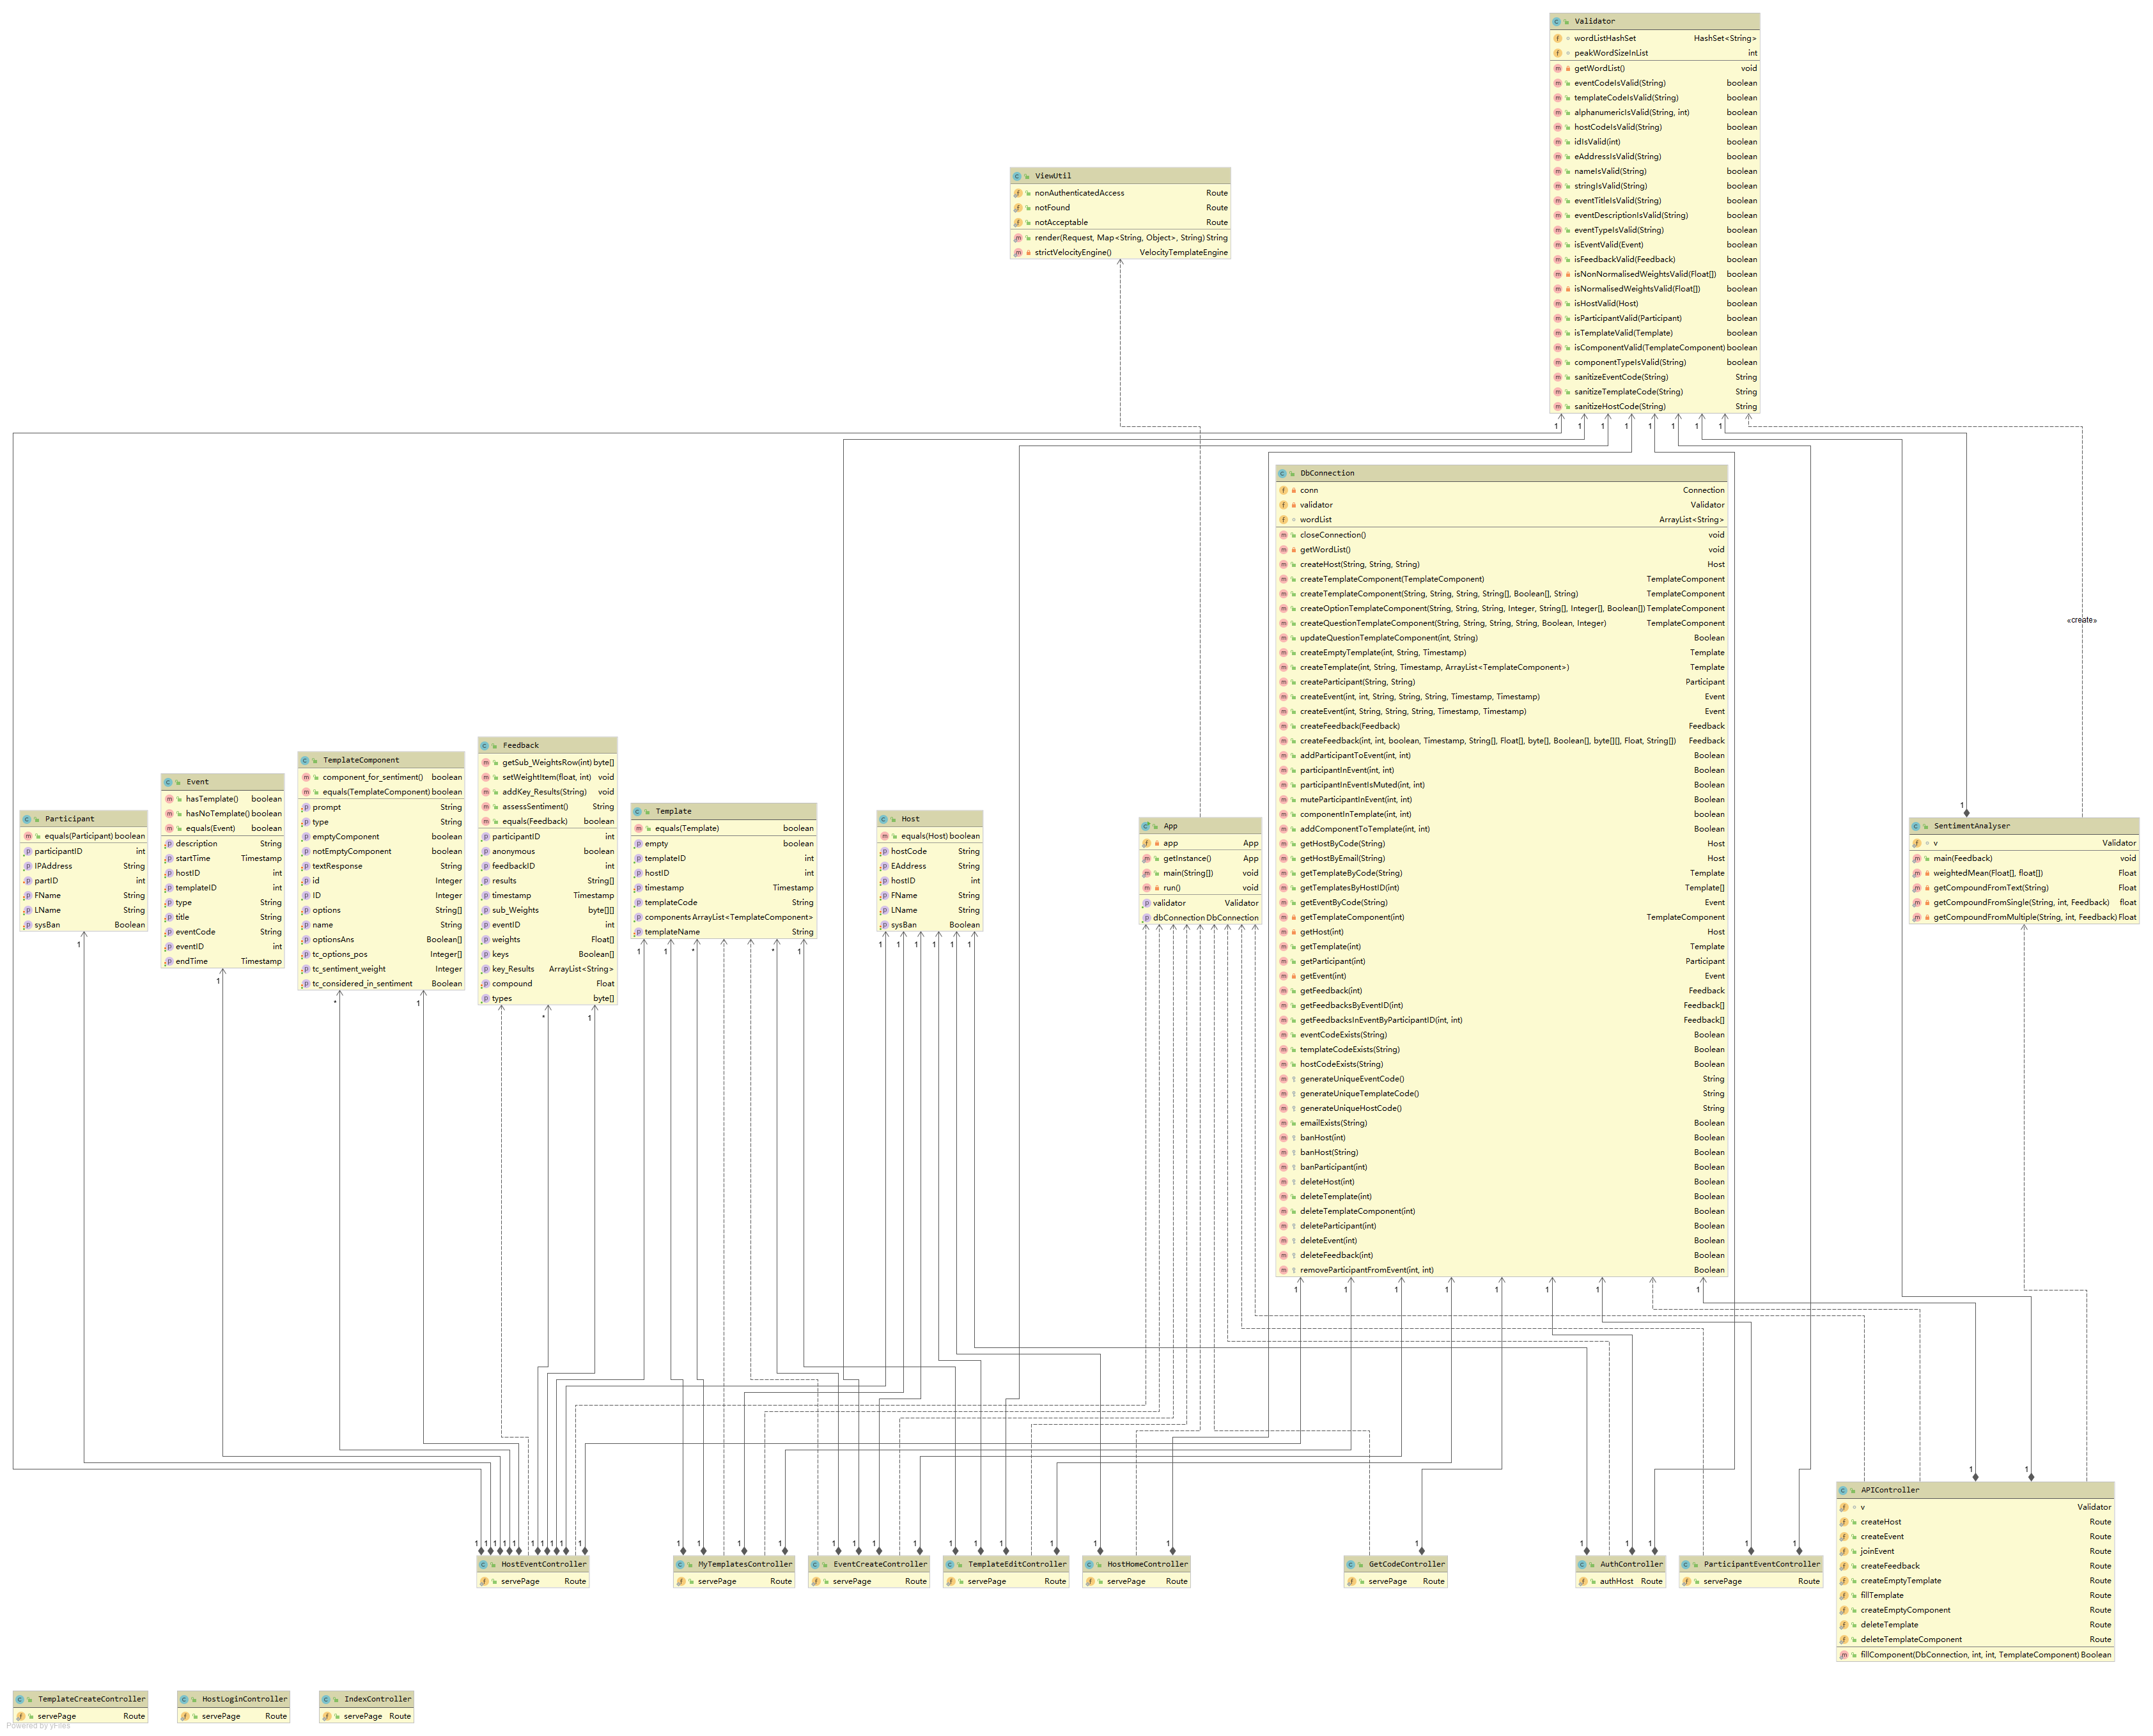
\includegraphics[width=\textwidth]{images/uml.png}
    \caption{\centering{Back-end UML class diagram; created with JetBrains IntelliJ IDEA.}\protect \\ (To view a larger version, see \autoref{fig:uml-sideways} in the Appendix.)}
    \label{fig:uml}
\end{figure}

\autoref{fig:uml} illustrates the back-end structure with an overview of the classes that comprise it. Each box in this diagram represents a class in the project. A dotted line between two classes represents that they are associated in some way and a line with a diamond on one side and numbers on both sides represents a more specific relationship. The class that has a diamond has a relationship with the other class and the numbers represents the amount of classes that the relation can hold.

\subsubsection{Database Modelling}

\begin{figure}[H]
    \centering
    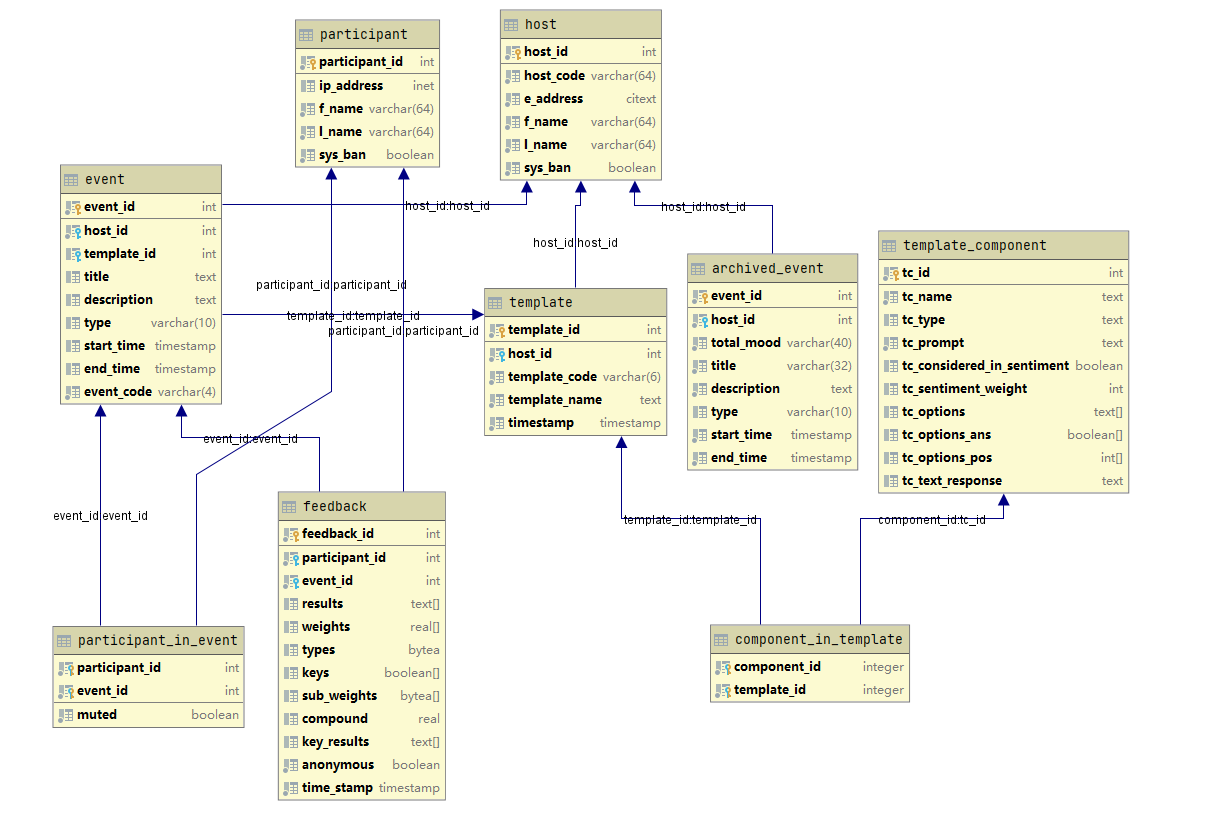
\includegraphics[width=5in]{images/db-model.png}
    \caption{Database dependency diagram; created with DataGrip.}
    \label{fig:db-model}
\end{figure}

\autoref{fig:db-model} shows the relations and keys in the database. Each block represents a relation in the database, Each arrow starting from a foreign key (blue key in blocks) and pointing to a primary key (yellow key in blocks), represents a link between these two keys. Newly added rows and relations replaced data in both feedback and template tables which helps represent those data in a more detailed and specific way and split different types of data clearly to reduce redundancy in queries. The component in template relation links components to their belonged templates and is used to reduce redundancy in storing data. These relations are in Third Normal Form - all the data elements in these relations are not only uniquely identified by the primary key but also independent of each other without any other functional relationships.

\subsection{Front-End} \label{sec:front-end}

\subsubsection{GUI Design}

GUI documentation captured from Google Chrome version \txttt{88.0.4}.

\begin{figure}[H]
    \centering
  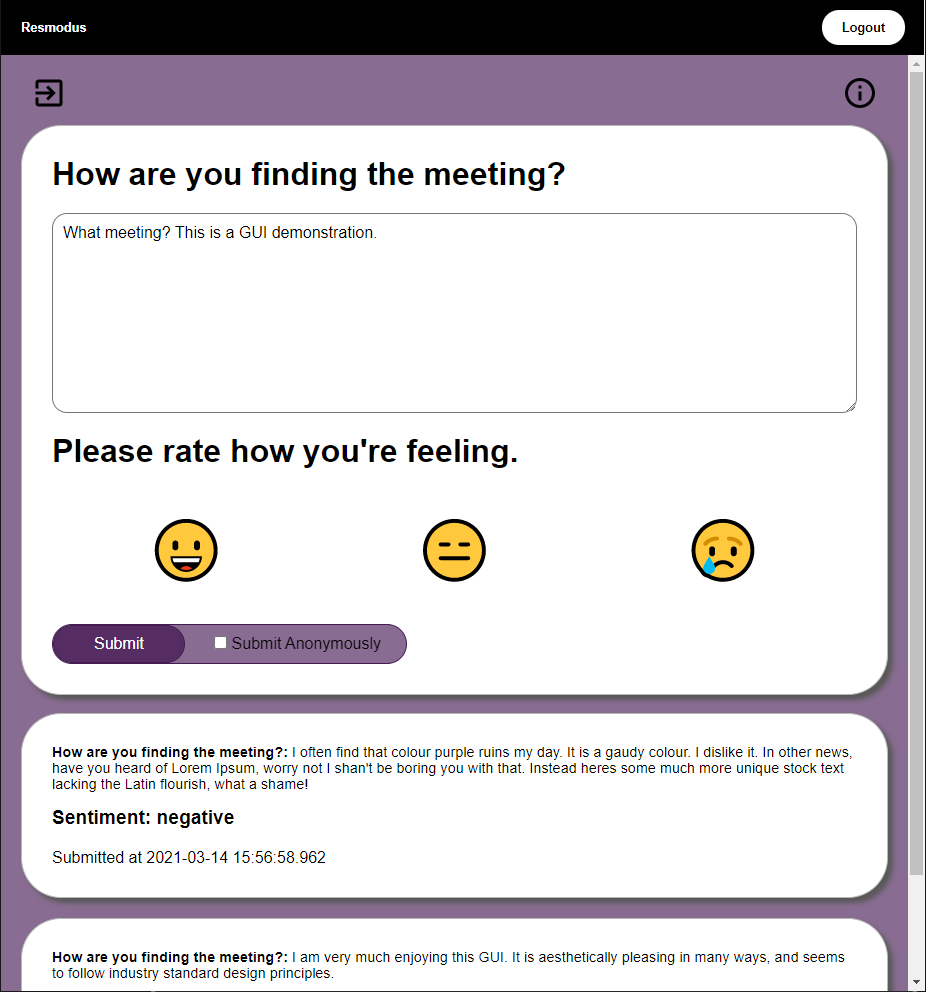
\includegraphics[width=.31\linewidth]{images/feedback_thin1.jpg}\hfill
  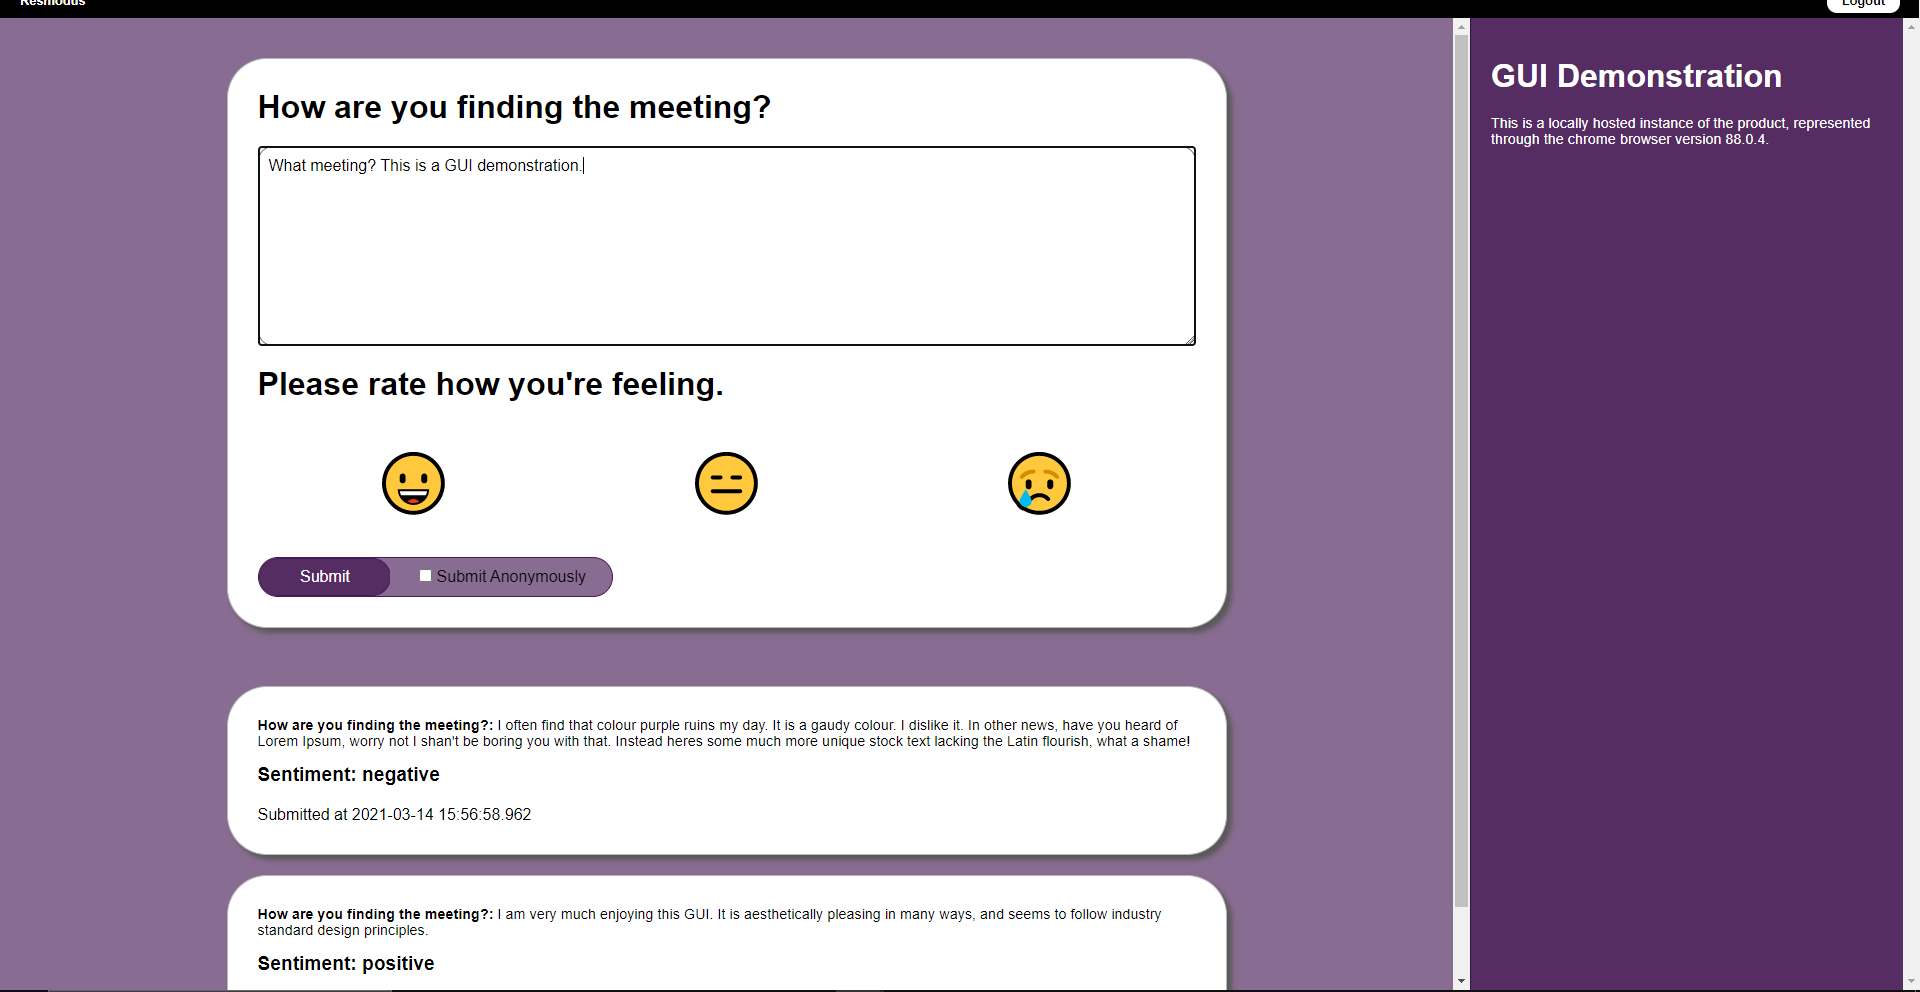
\includegraphics[width=.65\linewidth]{images/feedback_wide.jpg}\hfill
  \caption{Feedback submission page and event page containing feedback, across varying screen widths.}
  \label{fig:gui2}
\end{figure}

\begin{figure}[H]
    \centering
  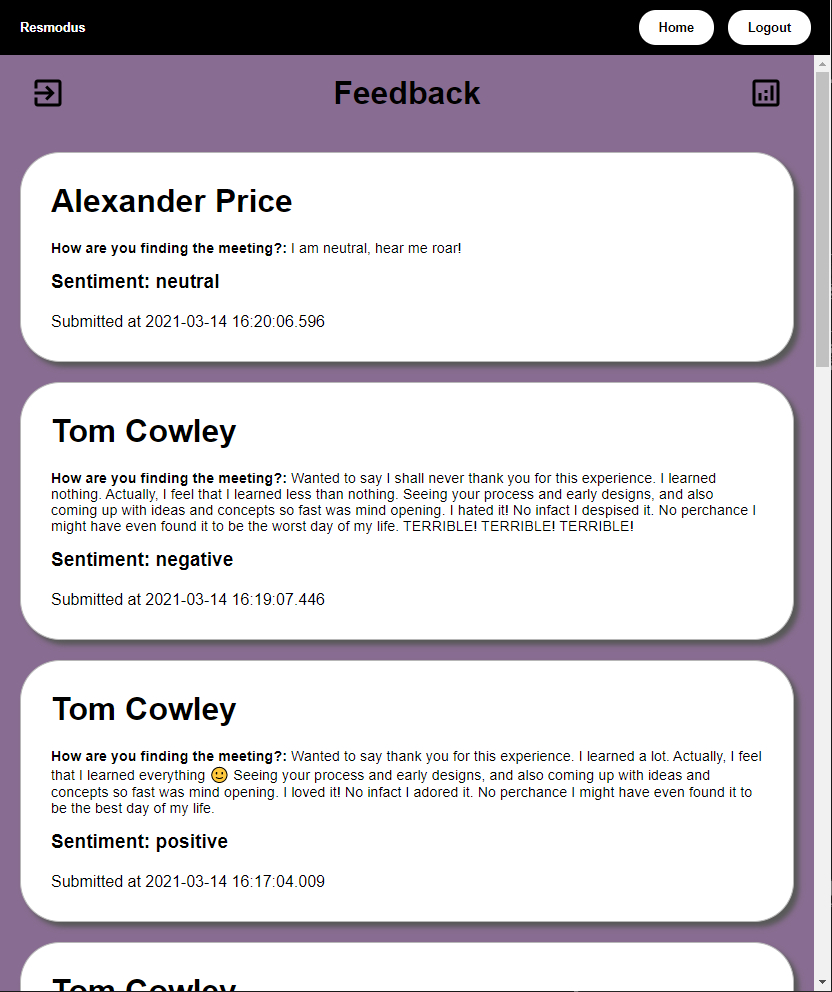
\includegraphics[width=.6\linewidth]{images/event_full_thin1.jpg}\hfill
  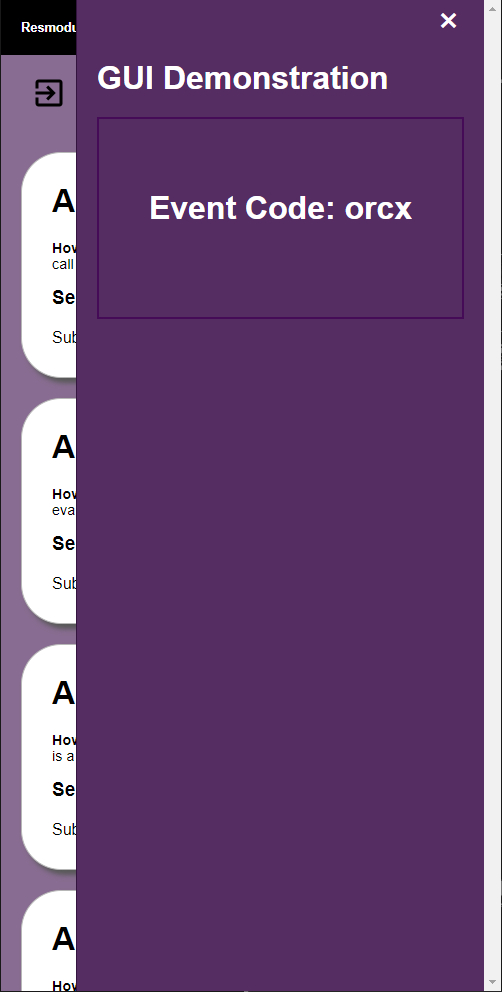
\includegraphics[width=.36\linewidth]{images/event_full_thin2.jpg}\hfill
  \caption{Feedback submission page and event page containing feedback, across varying screen widths.}
  \label{fig:gui3}
 \end{figure}

\begin{figure}[H]
    \centering
  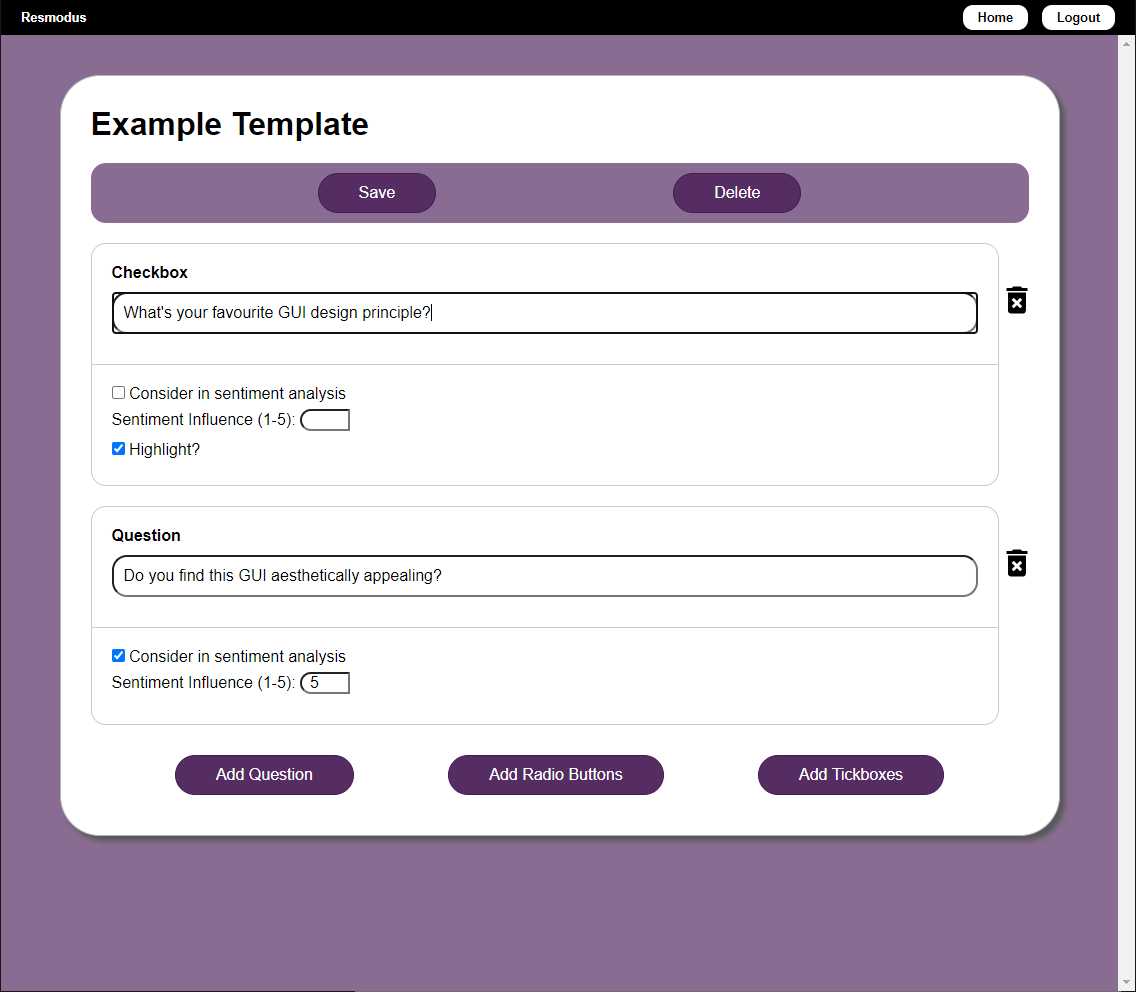
\includegraphics[width=.6\linewidth]{images/Template_Medium.jpg}\hfill
  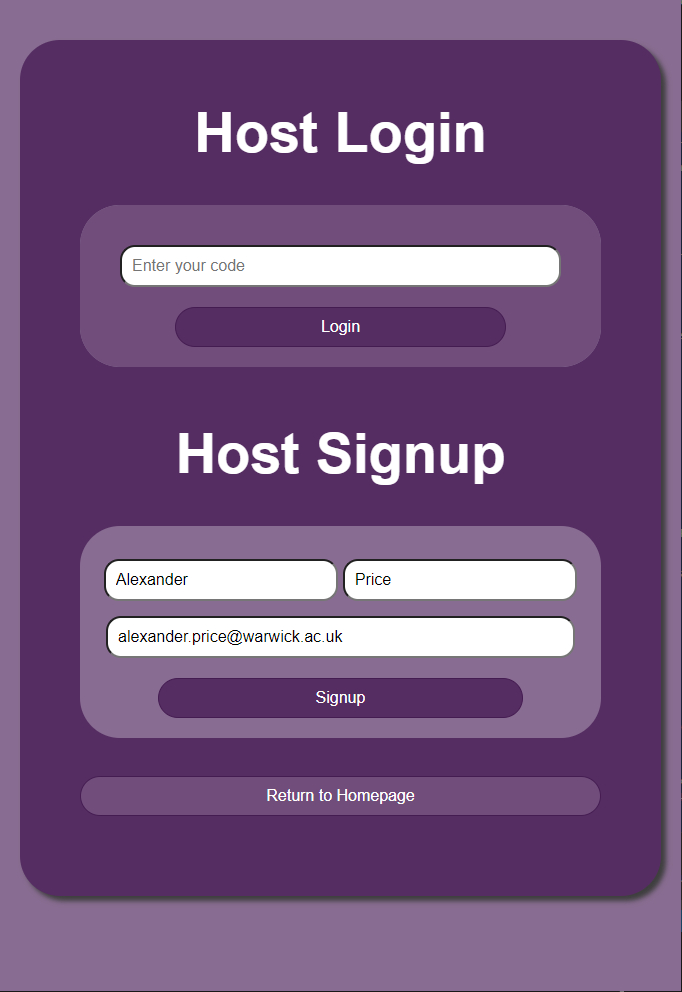
\includegraphics[width=.36\linewidth]{images/Host_Signup_Thin.jpg}\hfill
  \caption{Template creation page and host landing page, across varying screen widths.}
  \label{fig:gui1}
\end{figure}


All GUI designs follow the principles outlined the design document \cite{design-and-planning} and are styled consistently with the original mock-ups, this is consistent across screen widths from 1920px to 320px inclusive and across all the browser versions listed in the design document (see the testing section of this report for validation).\\

Maintaining spacing between interface elements promotes clarity, while separating interface elements with associated functions into areas that are spaced apart and differentiated by slight changes in colour promotes clarity and comprehensibility. Grouping interface elements with associated functions also minimises user hand and eye movements, promoting interface efficiency. Ensuring text is always placed on a background with a contrasting shade promotes readability which contributes to comprehensibility. \\

The function of interactive interface elements are clearly described either in text or using ‘IBM defined globally recognisable button icons’ \cite{ibm} licensed under Apache commons \cite{open}. An example is the icon used to view event details on the participant feedback submission page - an `i' within a circle, commonly understood to signify `information'. This ensures predictability and the use of recognised icons contributes to familiarity. \\

User actions are immediately acknowledged, promoting responsiveness. The testing section of this report validates this claim by testing interface latency. These interface design principles (and others discussed in the design document) \\

User interaction within the system is defined by forms, and user-input fields. Our product implements a system to display error messages against forms following the submission of invalid input. For an example error message, see \autoref{fig:error-message}: the case in which a participant is looking to join an event with an invalid event token. 

\begin{figure}[H]
    \centering
    \subfloat[\centering Before invalid submission]{{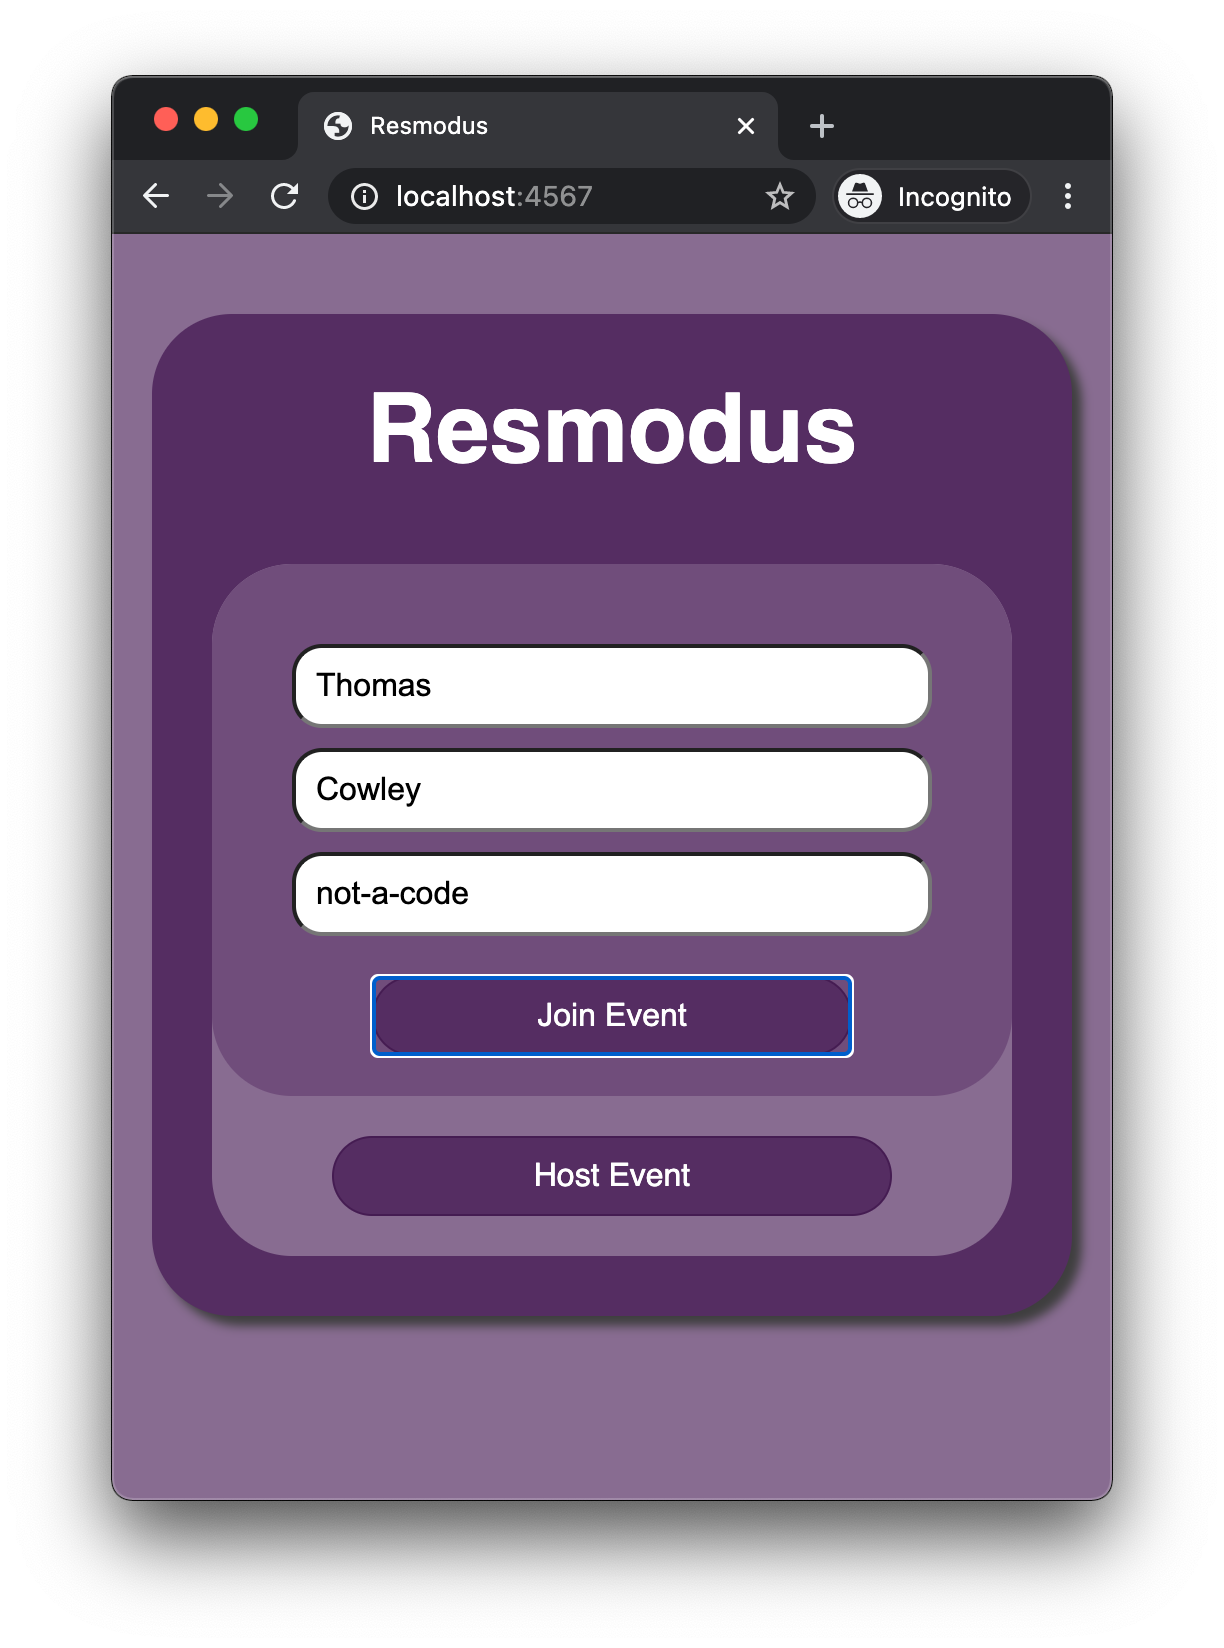
\includegraphics[width=0.5\textwidth]{images/join-event-error-p1.png} }}%
    % \qquad
    \subfloat[\centering Following invalid submission]{{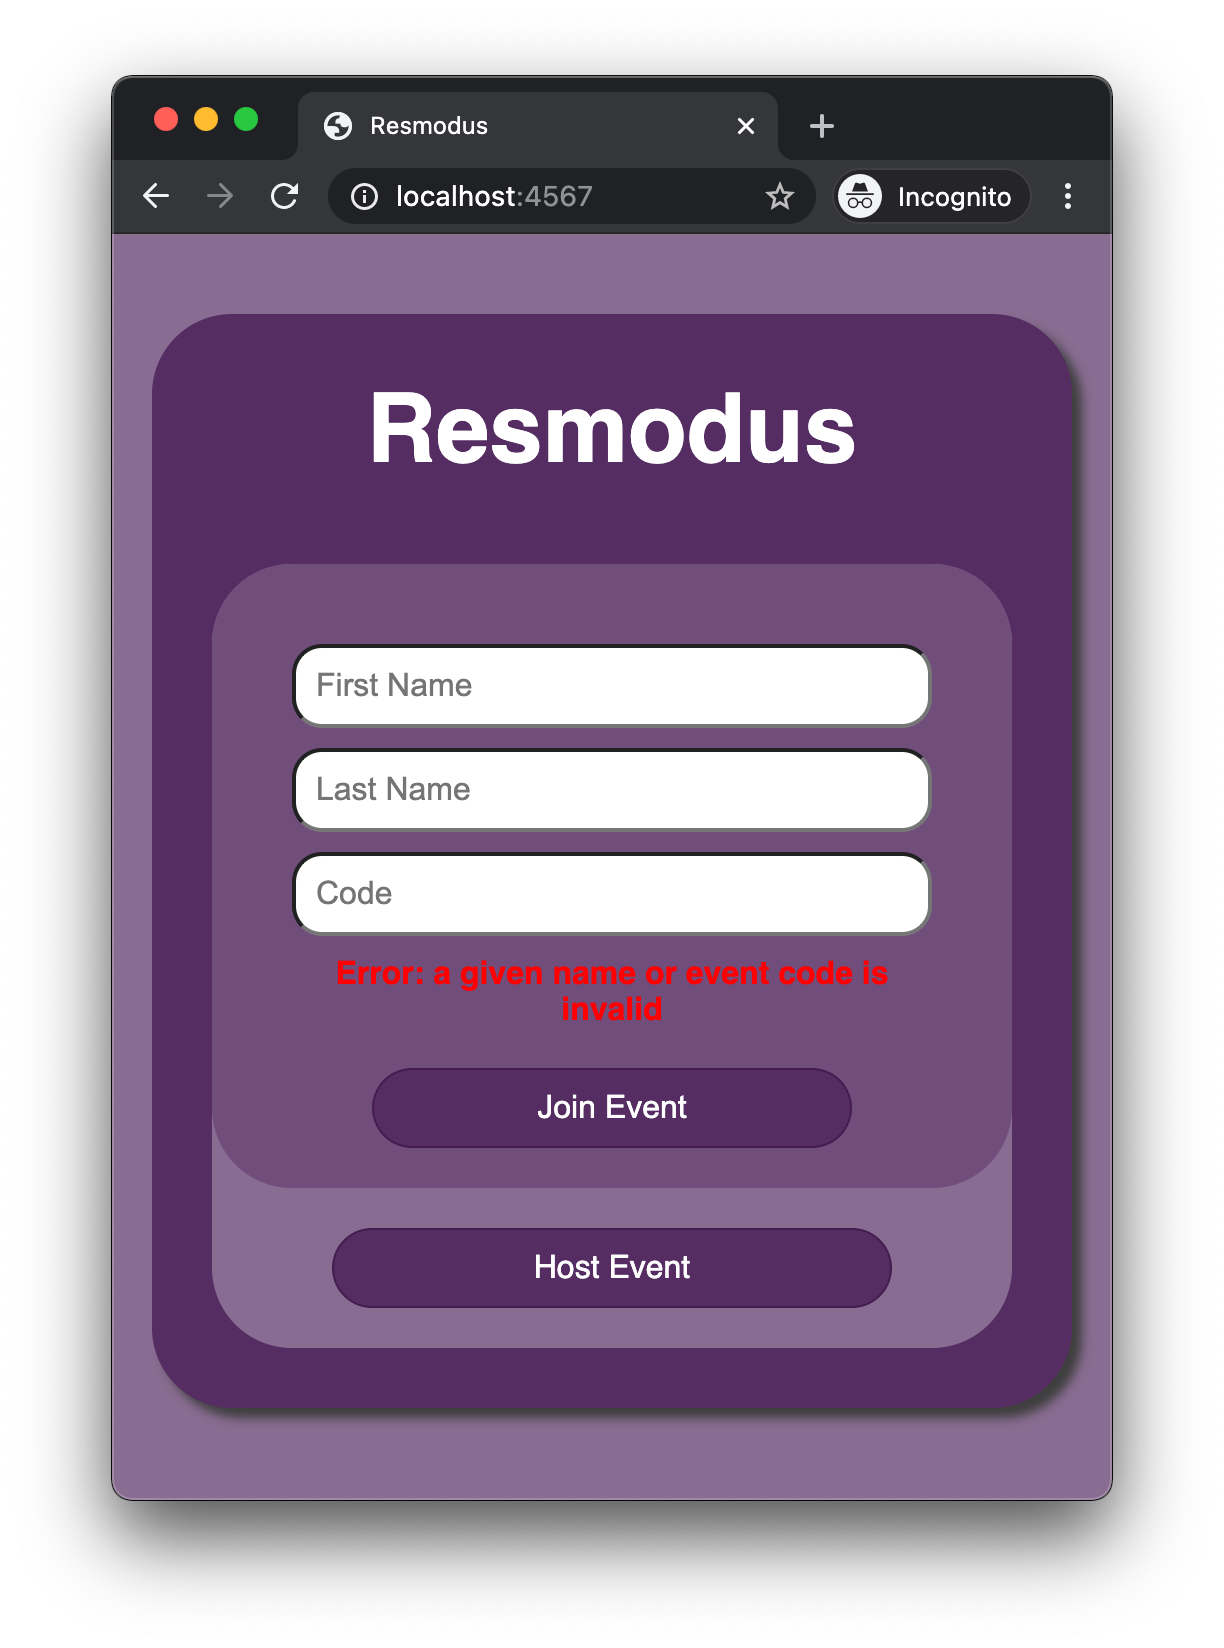
\includegraphics[width=0.5\textwidth]{images/join-event-error-p2.png} }}%
    \caption{An example error message within the system; at event joining}%
    \label{fig:error-message}%
\end{figure}

\subsubsection{GUI Implementation}

The user interface uses the Apache Velocity template engine. This allows for elements of web pages to be constructed dynamically using server-side Java code and variables. For instance, this allows the HTML header to be extracted to a separate file and remain consistent across all pages, reducing redundancies in the code. It is also used to add server-side content to pages by storing them in variables - for example, \texttt{/host/home} can display a user's name, and the participant feedback page can dynamically create a form based on the event's selected template.\\%(double check this? can the software do this, should we say this?)

Pages are defined using HTML, which specifies the content of the interface, dividing it into content areas with `tags'. CSS rules are applied to these areas, styling them to fit the GUI design (see the design document \cite{design-and-planning}).\\

Responsive styling is utilised in the CSS - this allows the page elements to change styles at certain screen widths. This ensures that the user is able to access all interactive UI elements and that the interface remains visually stable at all screen widths. This has been developed and tested from 320px to 1920px inclusive. Details on testing can be found in the Front-End \& UI Testing section. The Flexbox and Grid CSS technologies are utilised where applicable, allowing for easier responsive styling. For example, in \texttt{/event/participant/feedback}, a grid is used (on desktop) to split the page into two sections. CSS styles developed for some pages are reused in other pages where possible. This promotes a sense of consistency throughout the GUI and reduces the size of the style sheets.\\

JavaScript is utilised in the pages used to view events to handle the event description/analytics section. On desktop, this is held in a static section that takes up approximately a third of the page - however this is not feasible on mobile. So a separate slide-out menu is used, and JavaScript is utilised to make this appear and disappear when a button is pressed. The desktop section is hidden and the mobile section made visible with CSS once the screen falls below a certain width, and vice versa.\\

\subsection{Application Programming Interfaces}

\subsubsection{API Endpoints: GET listeners}

The system back-end implemented controller classes corresponding to each front-end page. These controllers contain public routes, mapped to GET requests for site pages. These routes serve front-end pages to the user, however include intermediate steps to prevent errors. Where necessary, sessions are checked to be live, request parameters and session attributes are checked to ensure their collection, validity, and existence within the database. These checks also form as a basis for page authentication: if, and only if, authenticating variables are set within the current session can the current user have access to the page. \\

Page serving routes also are the point of interface between the back-end APIs and the front-end pages. Each dynamic front-end page makes use of the Velocity framework (see \ref{sec:front-end}); these routes populate page variables with server-side data. This system includes that used to populate error messages within pages. Once the page model is constructed session stored messages are cleared and the front-end page is rendered using the Velocity template-renderer. 

\subsubsection{API Endpoints: POST listeners}
\subsubsubsection{Authenticating}

The system back-end implemented back-end route serving as an API that authenticates hosts. The submission of a host login form (containing just a host's token) is sent to the authenticate host API, in the form of a route object. The route retrieves the sent host code (from the request body), ensures said host code is valid, and then checks if the code exists within the system database. Only once all conditions are met is the host retrieved and stored in a user-local session. Note that the presence of the host object within the session acts as a basis for authentication across all routes. Finally, the host authentication API redirects the response to the host homepage. 

% class for authenticating host by host code provided. It will start a session for other non-Authenticating post and get methods to acquire host information and detect unauthenticated access to avoid.

\subsubsubsection{Non-Authenticating}

The system back-end implemented an \texttt{APIController} class storing each POST API endpoint listener (excluding authenticating methods). This controller contains all the public Route objects which process form data, sent via POST requests. These APIs first establish if the request came from an authenticated source, if appropriate; this is done via accessing session variables. Following this, form data is established to exist and collected; only then are request attributes validated with the system validator, and tested in the database for their existence. This order ensures minimal database interaction since any invalid data will be flagged prior to any database transaction; minimizing the number of database queries improves both the program latency, and system scalability. Following data validation, some action is performed on the data: be this a database interaction or some computation. If, and only if, each step has been successful is the user redirected to the following page. If at any point during the sequence of steps a condition fails, the user is redirected to the original page with a populated error message, such as those outlined in \autoref{fig:error-message}. 

Our system has implemented a large section of API endpoints within \texttt{APIController}: 

\subsection{Object Validation}

System object validation was delegated to the \texttt{Validator} class. Since this validation class is responsible for object validation, this conforms with the single-responsibility principle \cite{srdp}. Each system object, such as Templates, Feedback, etc., has a dedicated, publicly accessible method assessing its validity - a process assessing the validity of each object attribute value. Some methods, such as template components, have different interpretations within the system; its validity checking method therefore considers each case and checks internal attributes accordingly. \\

These validity checking methods have been developed in a scalable manor and make use of linear nesting over branched nesting to reduce complexity and improve readability. Additional conditions against fields can be appended (making this format scalable), and future developers can place debugging output within statement bodies to understand what is causing invalid objects. 

\subsection{Database Interaction}

The interaction between our application and database server is realised using \texttt{JDBC} \cite{jdbc}. The class \texttt{DbConnection} creates a connection to the database server and provides all the methods that can store and retrieve data. This class is initialised when the app starts running and can be called using the instance stored in the app. These methods can be sub-divided by function. \\

The creation methods take valid input values of each type of objects and stores them into the database. They return the stored object representation if it is stored successfully and null otherwise. The retrieval methods take valid IDs or Codes that recognise each type of objects and finds them within the database. These methods return the object if it is stored in the database and null if not. The deletion methods take valid IDs or Codes that recognise unique instance of each type of objects and deletes them in the database. They return \texttt{true} if it is found and deleted successfully and \texttt{false} if not. \\

The existence checking methods take valid codes that recognise unique instance of each type of objects and checks whether it is duplicated. They return \texttt{true} if it is already exists and \texttt{false} if not. The token generation methods generate a unique code to distinguish instances of objects. They return a unique object code that has been checked its corresponding existence checking methods. The mute object method takes valid IDs, codes or email addresses and sets a mute flag within the database against said object. They return \texttt{true} if it is found and muted successfully and \texttt{false} if not.\\

\subsection{Token Generation}

\subsubsection{Authentication Tokens} \label{auth-tokens}

To simplify host authentication, the system uses private authenticating host tokens. These are generated following host sign-up completion, then displayed to the user within a dedicated host token display page. Since this host token serves to uniquely authenticate hosts, a token that is both strong, and memorable, and unique is required. Host tokens are generated using the system word-list (containing over five hundred unique words); we define a host code as a string of four dash-separated words from the system word list (note that this directly corresponds with our plan outlined in \cite{design-and-planning}). An example valid host token within the system is \texttt{winter-yesterday-vegetable-weather}. \\

These tokens can be considered strong since the system interprets over 100 billion ($578^4$) unique host tokens; the chance of any valid host-code being guessed by a malicious user is infeasible.\\

The process of generating unique host tokens requires database interaction, and as a result, host code tokens are allocated to new hosts at the point of host object creation within the database; this has been done to further simplify and abstract host creation. 

\subsubsection{Non-authenticating Tokens}

Non-authenticating tokens provide a user-readable method to identify events and templates. 
These tokens have been implemented in accordance with our design outline: 
both tokens are case-insensitive alpha-numeric codes, with event and host tokens being of length four, and six, respectively. For example, a valid event code within our system could be \texttt{a1b2}, and a valid template code: \texttt{a1b1c2}. Tokens are used by the system front-end to choose events and templates. \\

These tokens are generated using database dependent methods, since any randomly generated token must be unique (therefore not colliding with existing tokens). Tokens are generated at the point of object creation within the database connector to simplify and abstract object creation. 

\subsection{Core Objects}

\subsubsection{Implementation Principles}

These principles are applied specifically to classes listed in this Core Objects section, although they may be applied to other classes within the project where suitable.\\

To promote encapsulation, all fields within classes have been made privately accessible. Each class field can be selected and updated via dedicated get and set methods, all of which are publicly accessible. The get methods retrieve and return the value of their respective field; the set methods take data of the correct type and store it in the field. Some get and set methods are more complex, such those getting or setting a single item from an array type field.\\

Additionally, every class features a public \texttt{equals} method. This takes a separate instance of that class and returns true if and only if they are identical (i.e. if each internal attribute is equal). These methods exist primarily to facilitate testing.

\subsubsection{Event}

Events within the system are modelled using the Events class. Each event is associated with a unique identifier, an author (host) identifier, a unique event token, a title, description, type, and start and end times. The system recognizes both events without templates, and events with templates: only events with templates are associated with a template identifier. Events belongs to one of five types: lectures, seminars, conferences, workshops, and others; the type of an event is stored within its type attribute. 

\subsubsection{Host}

Hosts represent a subset of users within the system. They have exclusive privileges such as event and template creation. Within the system, hosts are modelled using the \texttt{Host} class. Each host has an associated identifier, unique token, email address, first and last name. This unique token (or \texttt{host-code}) serves as a unique authenticating token for the host; see \autoref{auth-tokens}.

\subsubsection{Participant}

Participants also represent a subset of the users within the system. Participants can join events made by a host and provide feedback on the event, and the host can see this feedback in real time. Within the system, participants are modelled using the \texttt{Participant} class. Each participant has a unique ID, first name, and last name. Participants are not required to make an account to join an event, they simply use an event code that is shared by the host and then provide their credentials.

\subsubsection{Feedback} \label{sec:feedback}

Every instance of the \texttt{Feedback} class represents (and stores data about) a real world instance of feedback submitted by a participant.\\

The ID of the feedback is an auto generated serial number which is determined by the order that it is stored in the database. The timestamp of the feedback is auto generated and stores when the feedback is received and processed by the app. The anonymous flag of the feedback is obtained by the status of a checkbox which participants can toggle to choose whether to submit their feedback anonymously.\\

The content of the feedback is stored across 5 arrays of equal length. Each item in an array refers to the same query in the template in a one to one relationship - this is consistent across the arrays. A string array, \texttt{results}, stores the feedback input by the user into a specific query. A byte array, \texttt{types}, holds the response format of the query that generated the result: either from a simple text input (question), from a set of predetermined answers with selection limited to a single answer (radio buttons), or from a set of predetermined answers with unlimited selection (checkboxes). In the first case, the result is stored as a plain-text string. In the second case, the index of the chosen answer is stored as a character (string), and in the third case the indexes of all answers chosen are stored as a word. All indexes for answers chosen are a numerical character between 0 and 4. A boolean array, \texttt{keys}, holds whether or not a result is a key result. A float array, \texttt{weights}, holds the host-defined weight associated with each query - the weight is used to determine the importance of its associated result when calculating sentiment. Each weight is an integer between 1 and 5 inclusive, and after the feedback is analysed for sentiment the value will be processed and set to a float between 0 and 1 inclusive. A byte array, \texttt{sub\_weights}, holds the host defined weight associated with each predefined answer within queries that utilise them.\\

The \texttt{compound} field stores the feedback's approval metric, a Float between 1 and -1 inclusive. Float is an object wrapped version of float - this was chosen to enable the field to hold a null value to represent a lack of sentiment. It is an estimation of the feedback's overall evaluative disposition, and is calculated using the results to the queries the host has designated as relevant to the sentiment. The \texttt{key\_results} field (a String array) holds the results to the queries the host has chosen to highlight in the mood. Together these two fields comprise the sentiment of the feedback.

\subsubsection{Templates and Components} \label{sec:templates}

Templates are modelled by the system as a store of template components. Templates are each associated with a unique identifier, an author (host) identifier, a unique template token, a template name, a timestamp from the point of creation, and an array list of template components.\\

Template components, or components, represent sections of a template; they model question input, radio input, and checkbox input within the template. Each component is associated with a unique identifier, a component name, a component type (e.g. question, radio, or checkbox), the state of the inclusion of said feedback in sentiment analysis, and a weighting for sentiment analysis (1-5). If the component is of the question type, then it is also contains a text response field. If the component is of a discrete type (such as radio or checkbox), then the component is associated with an options array, a positive scores array, and a corresponding option answers array, storing each provided option and the user selection state. These arrays store data in parallel: option data share a common index across these arrays. 
For an example component, consider a radio component requesting participant satisfaction within an event: a radio component could be populated with two options for feedback: satisfied, and unsatisfied. The corresponding option answer array is set at the point of feedback, with only one of the two elements in the array representing true. For checkbox components the options answer array does not have such restrictions: any number of options can be selected (this is the key distinction between components of type checkbox, and those of type radio). 

\subsection{Sentiment Analysis}

The class \texttt{SentimentAnalyser} takes a \texttt{Feedback} object. It retrieves data from the object and uses it to calculate the feedback's sentiment, which it stores in the \texttt{Feedback} object. Upon being called, the class checks if the \texttt{Feedback} object passed is valid (by calling a method from the \texttt{Validator} class), and in the case of an invalid feedback, an error message is posted and computation within this method halts.\\

It processes the values from the \texttt{weights} array held in the \texttt{Feedback} object, so that they all sum to 1, while maintaining the ratio between them. This is done so that they may be used to calculate a weighted mean. This is done by summing the weights then dividing each individual weight by the sum of all weights. The new weights are stored in the \texttt{Feedback} object (replacing the old \texttt{weights}).\\

Each item in \texttt{types} is inspected, and if the \texttt{weights} value of the same index is not 0, the item in \texttt{results} of the same index is passed to one of three compound calculating methods based on nature of the query that generated the result (as defined in \texttt{types}). The compound calculating method returns a Float value, which is stored in the float array \texttt{compounds}, with an identical index to the \texttt{results} value it was calculated from. The compound calculating methods return a Float for testing purposes, as during the testing the methods may return a lack of sentiment (null). This is not required during the running of the product, hence compounds is a float array.\\

The method \texttt{getCompoundFromText} performs natural language processing (NLP) on a plain-text string. The \texttt{BreakIterator} class (with a \texttt{UK} instance of the \texttt{Locale} class) is used to create an array list of the linguistic sentences that comprise the plain-text string. Each sentence is then individually analysed by the VADER NLP framework \cite{vader2}. The result of this is a float normalised between -1 and 1 inclusive. 

The compound score of each sentence is stored in a double array, and the standard deviation of the compound scores is calculated. Every compound score that falls within one standard deviation from 0 is excluded. This serves the function of excluding largely non-evaluative statements, as otherwise their inclusion would incorrectly bias the compound score towards 0. The mean of the remaining compound scores is calculated, the mean is returned.\\

The method \texttt{getCompoundFromSingle} calculates the compound score of a result generated by a query that takes a predetermined answer with selection limited to a single answer. It analyses the value of the result to determine the weight of the selected predetermined answer (stored in the field \texttt{sub\_weights} of the \texttt{Feedback} object). It then normalises the weight to between -1 and 1 inclusive. The method \texttt{getCompoundFromMultiple} does the same except it selects one or more weights (as the result can include one or more predetermined answers) and means them before normalising them. Both return the normalised value as a Float.\\

Once every result has had an associated compound score calculated, a weighted mean of all compound scores is calculated, and stored in the \texttt{Feedback} Object. Additionally every item in \texttt{results} designated as a key result is added to the \texttt{key\_results} array list in the \texttt{Feedback} object.

\subsection{Testing Framework}

\hypertarget{testing-and-validation}{%
\section{Product Testing and Validation}\label{testing-and-validation}}

\hypertarget{unit-testing}{%
\subsection{Unit Testing}\label{unit-testing}}

Development utilised unit testing at the point of development, as planned
in the Design and Planning Document \cite{design-and-planning}; unit
testing was carried out between sprint cycles one and six. Unit tests 
were applied to the Spark Java back-end \cite{web:spark} , and included: the database 
interaction methods (\texttt{DbConnTest}), the sentiment analysis 
methods (\texttt{SentimentTest}), and the validation methods (see 
\texttt{ValidatorTest}); these were developed in the form of JUnit 
tests against each publicly accessible method from the main source code, and are stored in \texttt{/app/src/test/}.\\

The unit testing follows the principles and methods outlined in the design document (as discussed below). The unit test were effective and consistently produced the correct results. Where appropriate our testing format was scalable: test data was held in data structures capable of holding multiple discrete data items, and these items were categorised by validity state. Additionally there was little labour cost for editing or expanding test data as the unit tests were dynamic. Where appropriate edge case checks were included in unit testing, such as those that considered blank, empty, and null fields.\\

\newpage

\subsection{Component Testing}

\begin{figure}[h!]
    \centering
    \subfloat[\centering Surefire report section  1]{{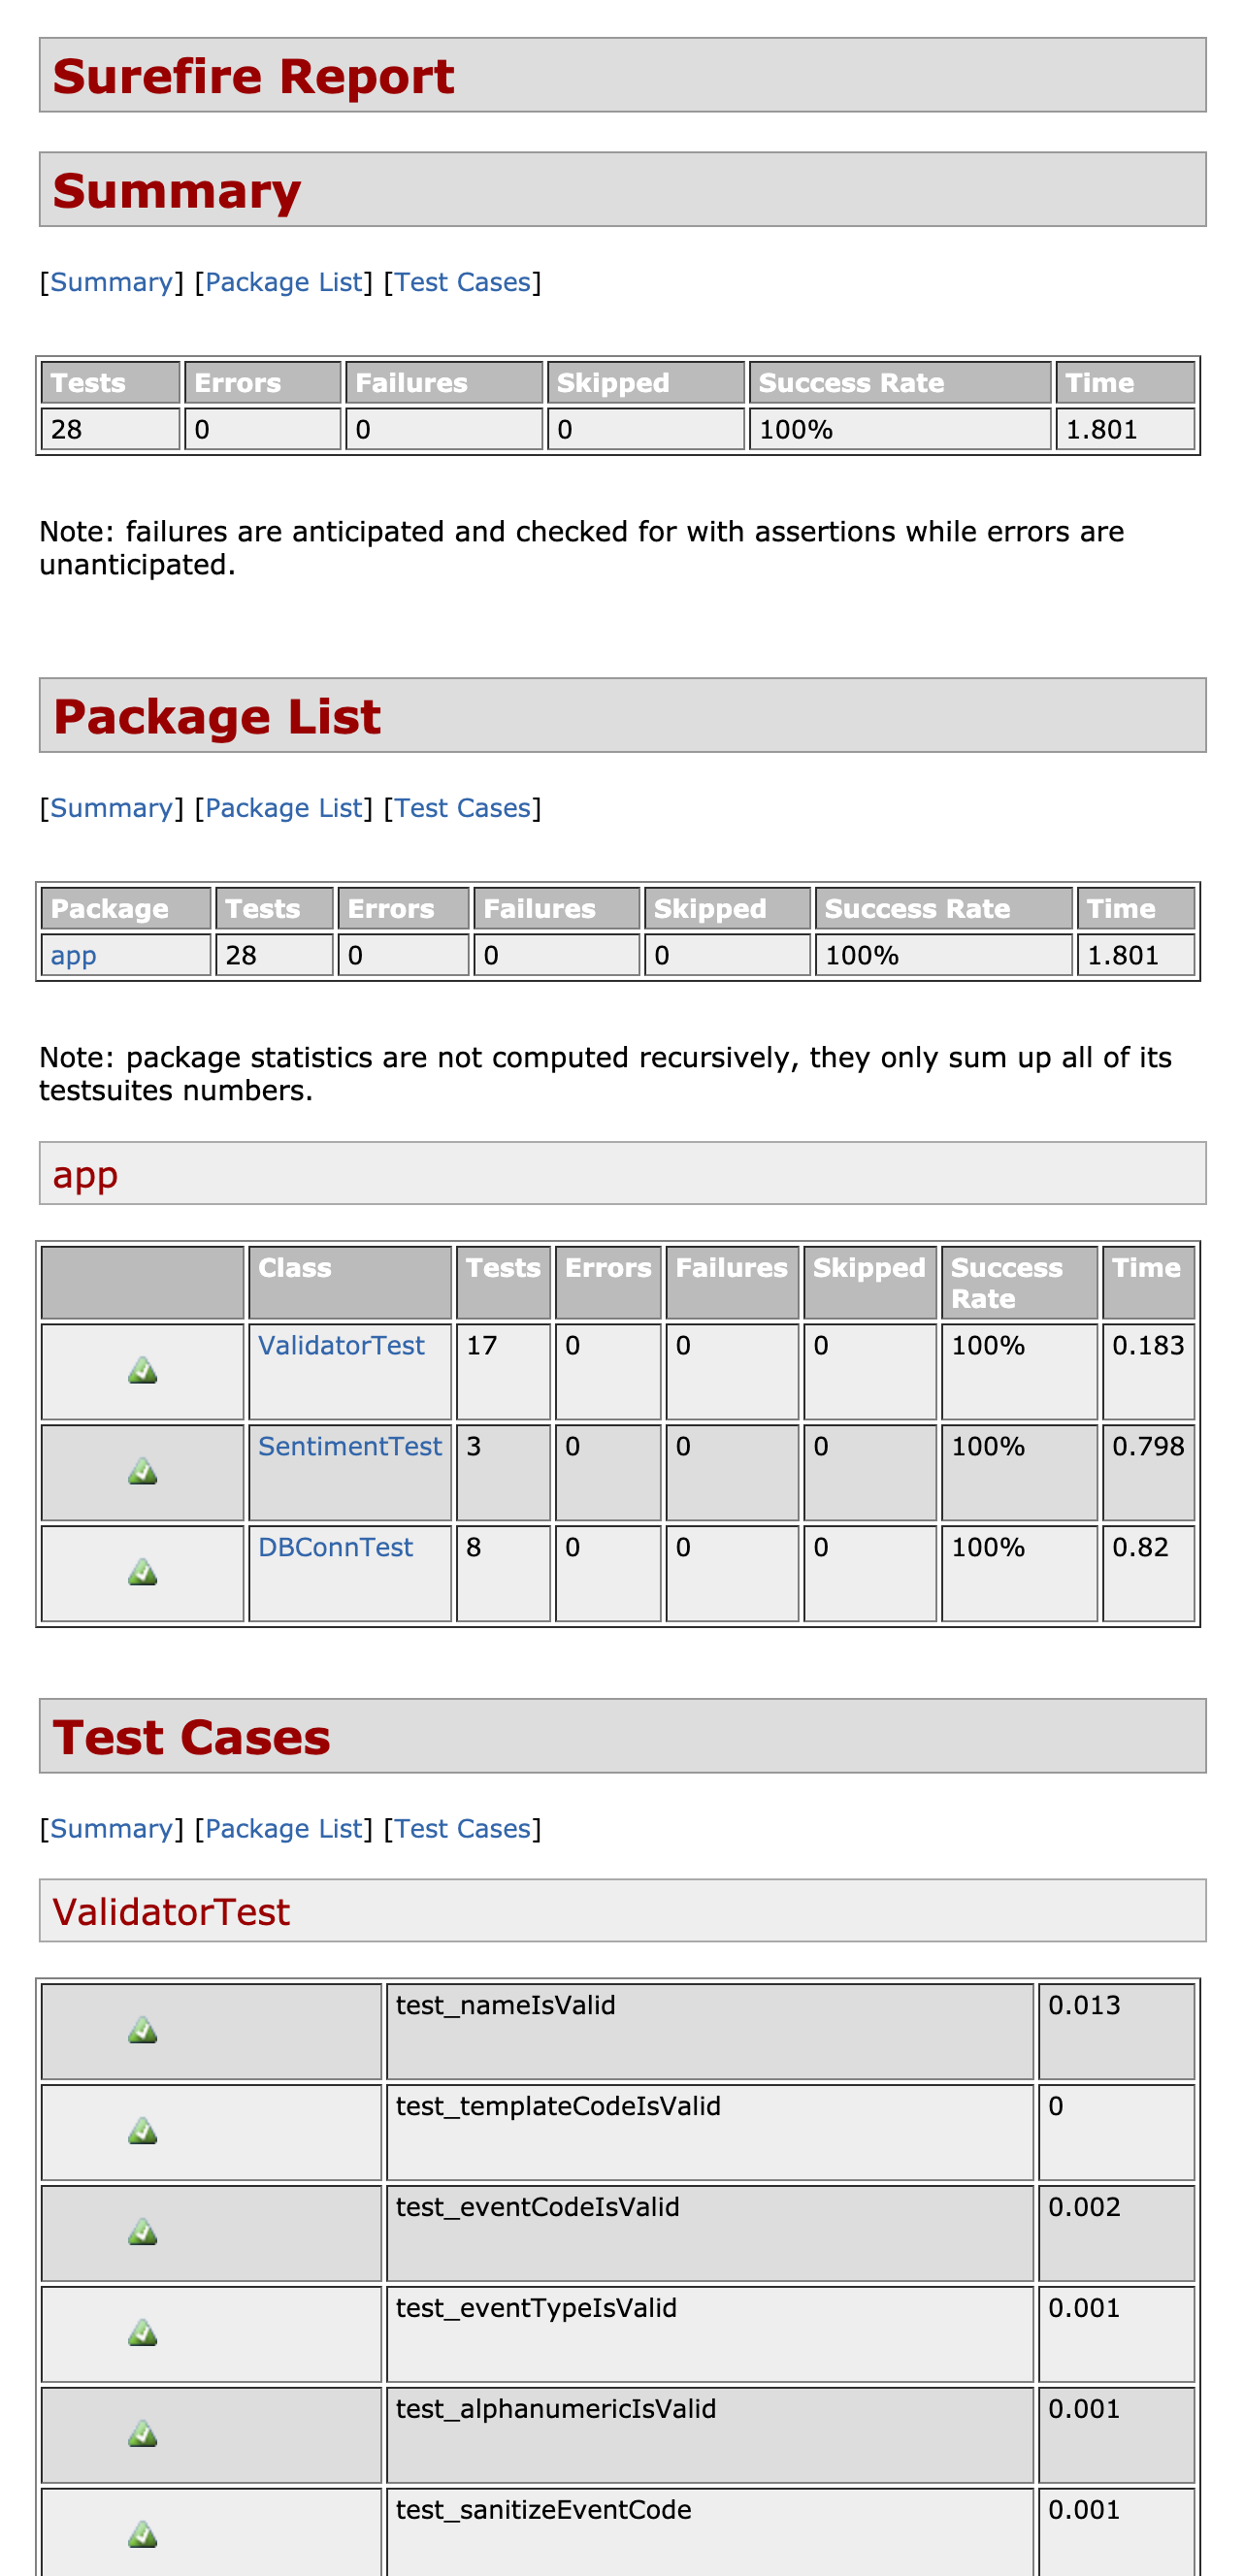
\includegraphics[width=0.5\textwidth]{images/mvn-report-p1.png} }}%
    % \qquad
    \subfloat[\centering Surefire report section  2]{{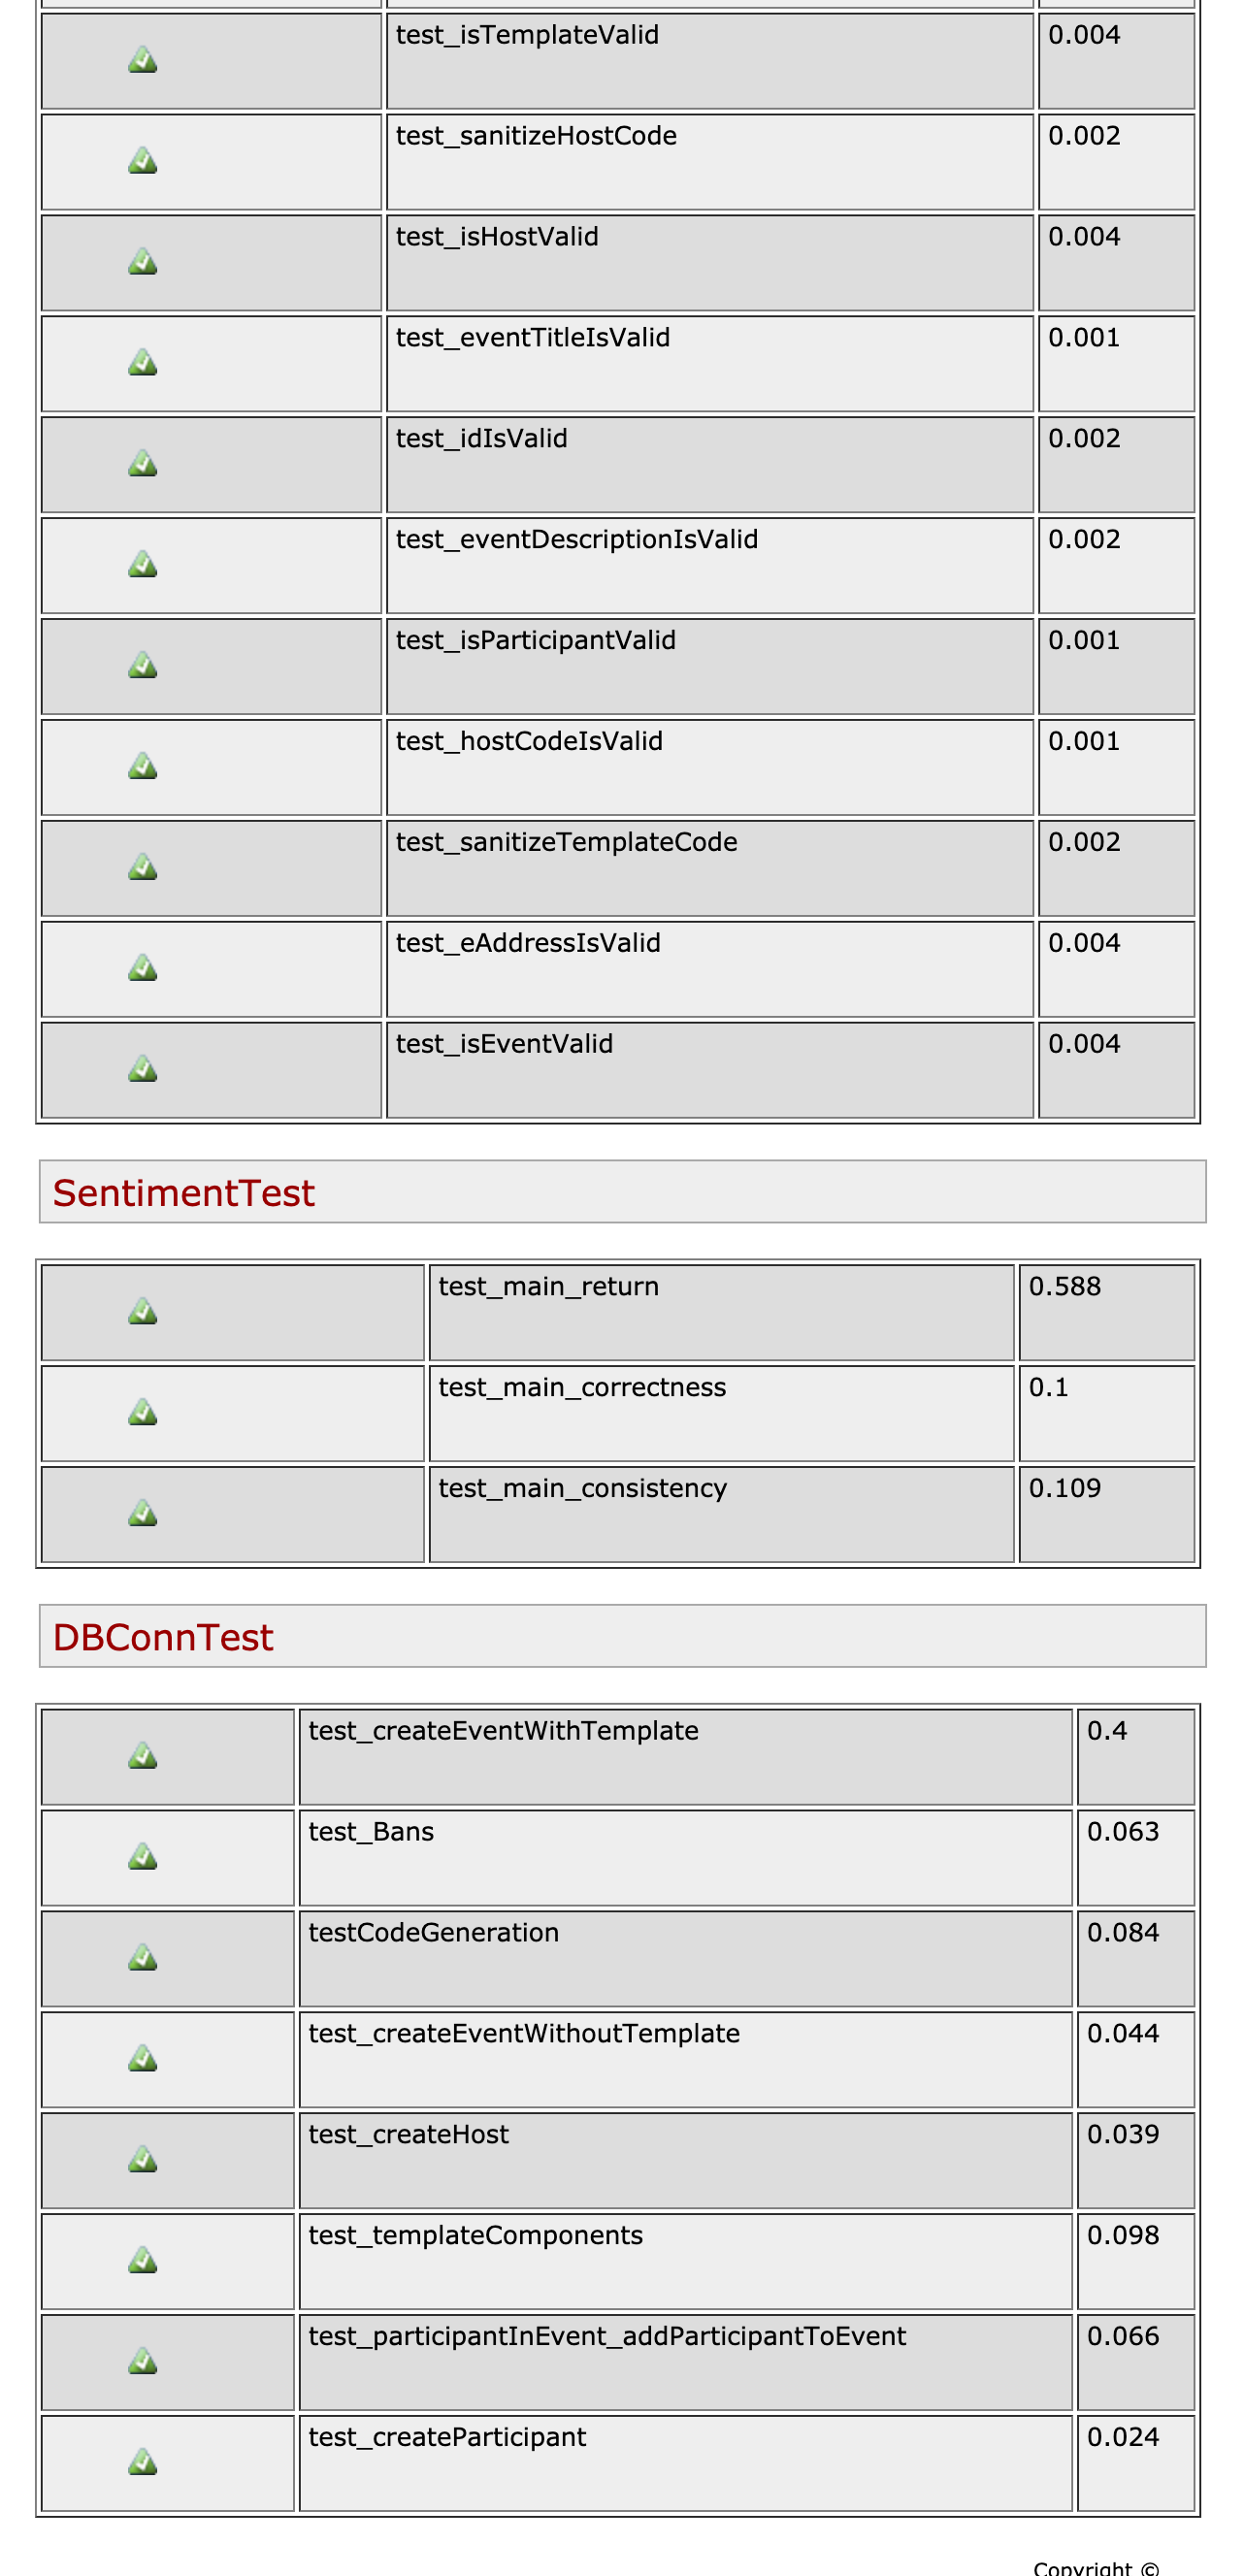
\includegraphics[width=0.5\textwidth]{images/mvn-report-p2.png} }}%
    \caption{Component testing report; generated with Maven Surefire \cite{surefire}}%
    \label{fig:testing-report}%
\end{figure}

Each back-end component: \texttt{DbConnection}, \texttt{Validator}, and \texttt{SentimentAnalyser} were subject to component-based usability tests to evaluate class and class method efficacy. This form of testing was suitable to our project due to our use of the model-view-controller (MVC) architecture, dividing our project into three core components. \\

The result of this 28 method test is depicted in \autoref{fig:testing-report}. \\

While each class passed its respective set of tests, and a large subset of internal public methods were assessed, these tests were not fully comprehensive. Some publicly accessible methods within \texttt{DbConnection} were not assessed due to time limitations during development. This is described in further detail in the Testing section of the Product Compromises section.

\subsection{System Testing}

\subsubsection{User Acceptance}
User Acceptance Testing as described in the design document \cite{design-and-planning} was performed, producing a user acceptance summary. This summary revealed that users were generally satisfied with the graphical user interface, although it could be confusing in some cases.\\

Users found it to be aesthetically appealing, and interface elements were clearly presented. When joining events and leaving feedback, users generally found the process intuitive. However they also reported that some of the more complex functionality was not directly explained, which lead to confusion. On the host side, the design suffered from a general lack of explanation of key features - negatively impacting the intuitiveness and time to learn. Users reported difficulties in particular with the template system and the login system. The login code system was hard to understand, and users commonly entered their email into the login box, demonstrating poor mistake avoidance. Users suggested that the solution incorporate clearer explanations of what things do, with the possibility of optional help boxes that could provide detailed explanations to confused users.

\subsubsection{Front-End \& UI}
The solution was tested for web standard compliance with the W3C Markup Validator \cite{web:w3c} and passed. The latency of all GUI interactions was tested, on a locally hosted instance. All GUI interactions happened within 300ms, which falls within the industry standard ‘good’ range for latency as documented by VictorOps \cite{victorops}.\\

To test device compatibility, all UI tests were performed on each of the mobile and desktop browser versions outlined in the requirements analysis document \cite{requirements-analysis} as well as across a variety of simulated screen sizes, ranging from a width of 1920px to 320px. In all cases the UI operated as expected and without error.

\section{Project Evaluation}

This section evaluates the product and the implementation process. The product is compared against the requirements \cite{requirements-analysis}, and its detriments as well as areas of potential improvement are discussed. The implementation process is evaluated primarily through the methodology and management utilised by the developers.

\subsection{Product}

\subsubsection{Requirements Analysis}
The full list of requirements can be found in the requirements analysis document \cite{requirements-analysis}.

\begin{enumerate}[noitemsep, topsep=0pt, leftmargin=9mm]
 \item[1.1 -] The must statement of this requirement is fulfilled by system testing, specifically component testing which demonstrates a web-app functions. Additionally front-end testing establishes the web-app is compatible with both desktop and mobile. The could statement of this requirement is unfulfilled.
  \item[2.1 -] This requirement is fulfilled, this is validated by \textt{testcodegeneration}, \textt{test\_hostCodeisvalid}, and \textt{test\_santizeHostCode} in component testing.
   \item[3.1 -] This requirement is fulfilled, this is validated by \textt{test\_isEventValid} in component testing.
 \item[3.2 -] This requirement is fulfilled, this is validated by \textt{test\_alphanumericIsValid}, \textt{test\_eventCodeisvalid}, and \\\textt{test\_santizeEventCode} in component testing.
 \item[3.3 -] This requirement is fulfilled, this is validated by \textt{test\_nameisValid} in component testing.
 \item[3.4 -] This requirement is fulfilled, this is validated by {isFeedbackValid} in the \texttt{Validator class} 
 \item[4.1 -] This requirement is partially fulfilled, validated by robustness as described in product description.
 \item[4.2 -] This requirement is unfulfilled.
 \item[4.3 -] This requirement is partially fulfilled, validated by user acceptance testing.
 \item[5.1 -] This requirement is partially fulfilled, although has not been validated due to product comprises associated with testing, and thus shall be considered as unfulfilled.
 \item[5.2 -] This requirement is fulfilled, verifiable by system testing.
 \item[6.1 -] This requirement is fulfilled, this validated by user testing.
 \item[6.2 -] This requirement is partially fulfilled, although has not been validated due to product comprises associated with testing, and thus shall be considered as unfulfilled.
 \item[7.1 -] This requirement is fulfilled, verifiable by code-base inspection.
 \item[7.2 -] This requirement is partially fulfilled, verifiable by code-base inspection.
 \item[7.3 -] This requirement is fulfilled, verifiable by code-base inspection.
 \item[8.1 -] This requirement is unfulfilled. 
 \item[8.2 -] This requirement is fulfilled, verifiable by document and code-base inspection. 
 \item[8.3 -] This requirement is fulfilled, verifiable by front end testing. 
\item[9.1 -] This requirement is fulfilled, verifiable by design and planning document inspection.
\item[10.1 -] This requirement is fulfilled, verifiable b\texttt{test\_eventDescriptionIsValid}, \texttt{test\_isEventValid}. 
\item[10.2 -] This requirement is fulfilled, verifiable b\texttt{test\_eventDescriptionIsValid}, \texttt{test\_isEventValid}. 
\item[11.1 -] This requirement is met by the system; this has been verified by both user acceptance testing and internal unit testing methods such as \texttt{test\_createEventWithTemplate()} within the testing class \texttt{DbConnTest}.
\item[11.2 -] This requirement is met by the system (and has been implemented with template components); this has been verified by both user acceptance testing and internal unit testing methods such as \texttt{test\_createEventWithTemplate()} within the testing class \texttt{DbConnTest}.
\item[11.3 -] This requirement is met by the system (and has been implemented with template components); this has been verified by both user acceptance testing and internal unit testing methods such as \texttt{test\_createEventWithTemplate()} within the testing class \texttt{DbConnTest}.
\item[12.1 -] This requirement is met by the system and has been verified by all 3 component tests under \texttt{SentimentTest}.
\item[12.2 -] This requirement is not met by the system; see product compromises.
\item[13.1 -] This requirement was fulfilled by the system. This is verified by user acceptance testing. 
\item[13.3 -] This requirement was not fulfilled by the system; see product compromises.
\item[13.3 -] This requirement was not fulfilled by the system; see product compromises.
\item[13.4 -] This requirement was not fulfilled by the system; see product compromises.
\item[14.1 -] This requirement was not fulfilled. See product compromises.
\item[14.2 -] This requirement was not fulfilled. See product compromises.
\item[14.3 -] This requirement was not fulfilled. See product compromises.
\item[14.4 -] This requirement was not fulfilled.
\item[14.5 -] This requirement was not fulfilled.
\end{enumerate}

\\The product fully fulfilled: 11/14 must requirements, 10/16 should requirements, 0/5 could requirements, and 0/1 won't requirements. However 5 should requirements were partially fulfilled. Overall the product failed at satisfying the requirements, as some must and several should requirements were not fully fulfilled. Although the product remains functional and fulfilled the majority of requirements, including 79\% of must requirements - in terms of satisfying the requirements the product is a minor failure. 

\subsubsection{Potential Improvements}

The largest detriment of the product was the features and systems not developed due to design comprises. Specifically the loss of some aspects of dynamic templates, mood metrics, and testing. These severely impacted the viability of the product, making it partially non-functional when compared against the customer needs and desires. Compromising features that fulfilled should or could requirements such as; native mobile applications, archived events, misuse prevention, and security - reduced the quality and efficacy of the product. Some compromises did not directly effect requirements but still were detriments to the product, such as dynamic URLs, the comprise of which reduced user accessibility and negatively impacted code distribution. Most comprised features are already partially if not mostly developed, and thus improving the product with further development would be incredibly labour efficient.\\

The products design and implementation was lacking in some key areas. Javascript could have been utilised in more areas to make the GUI more dynamic and responsive. The design could have stored data in Feedback objects using template component objects. This would have reduced total computation by reducing data conversions and parsing, while introducing more consistency, and requiring less labour to develop.\\

The original design (and all subsequent evolutions) lacked a method to sort and search feedback. This would have contributed to fulfilling requirements associated with the quality of the user experience. Additionally the requirements should have evolved to incorporate this feature as a should requirement. The lack of this feature deprives host users of non-cumbersome access to feedback once feedback submissions reach a large volume. This is a serious detriment against the requirements, design, and product.\\

While our authentication method is well suited to the system as a proof of concept, implementing an industry-standard compliant system (such as OAuth-2 \cite{web:oauth}) would be justified within any future development. Similarly other security features could be expanded, such as distribute denial of service attack protection and more comprehensive malicious user protection.

\subsection{Methodology \& Management}

The initial methodology was well conceived and effective. However, management failed to utilise adaptive agile principles. Thus, the methodology was nonreactive to issues caused by a flawed design and poor coordination. Furthermore, methodology was continually evolving in unproductive ways until the project became largely unproductive. At this juncture, management were able to create an effective methodology, supported by robust coordination/communication practices. However, they failed to mitigate against the attritional effect of labour-intensive development over a 12 day period. This resulted in major product comprises, and ultimately the failure of the project.

In the first sprint cycle, management effectively established documentation and communication frameworks, but was unable to evolve these to suit changing team needs until late into development. However, late into development, management enforced a highly efficacious group development system with thorough and efficient documentation.

Both the management and methodology improved over the course of the project. Had the team started the project with the experience and knowledge it acquired by the end of it, then perhaps they would have successfully adapted to the changes and taken advantage of the opportunities presented by design evolution.

\subsection{Conclusion}

The project started with valid and high quality requirements, which were used to create a design which lacked detail. The satisfactory project methodology was unable to adapt to issues caused by the design and perpetuated by poor coordination between developers. After a long period of unproductive development, the project compromised on its product and developed an effective methodology. However, not enough project time remained, so the product and its testing and validation were further compromised.
\\The product is a functional failure - it fulfills many of the customer's needs and desires, but not enough of them to justify its existence.

\printbibliography[heading=bibintoc]

\newpage

\section{Appendix}
\appendix

\begin{figure}[H]
    \centering
    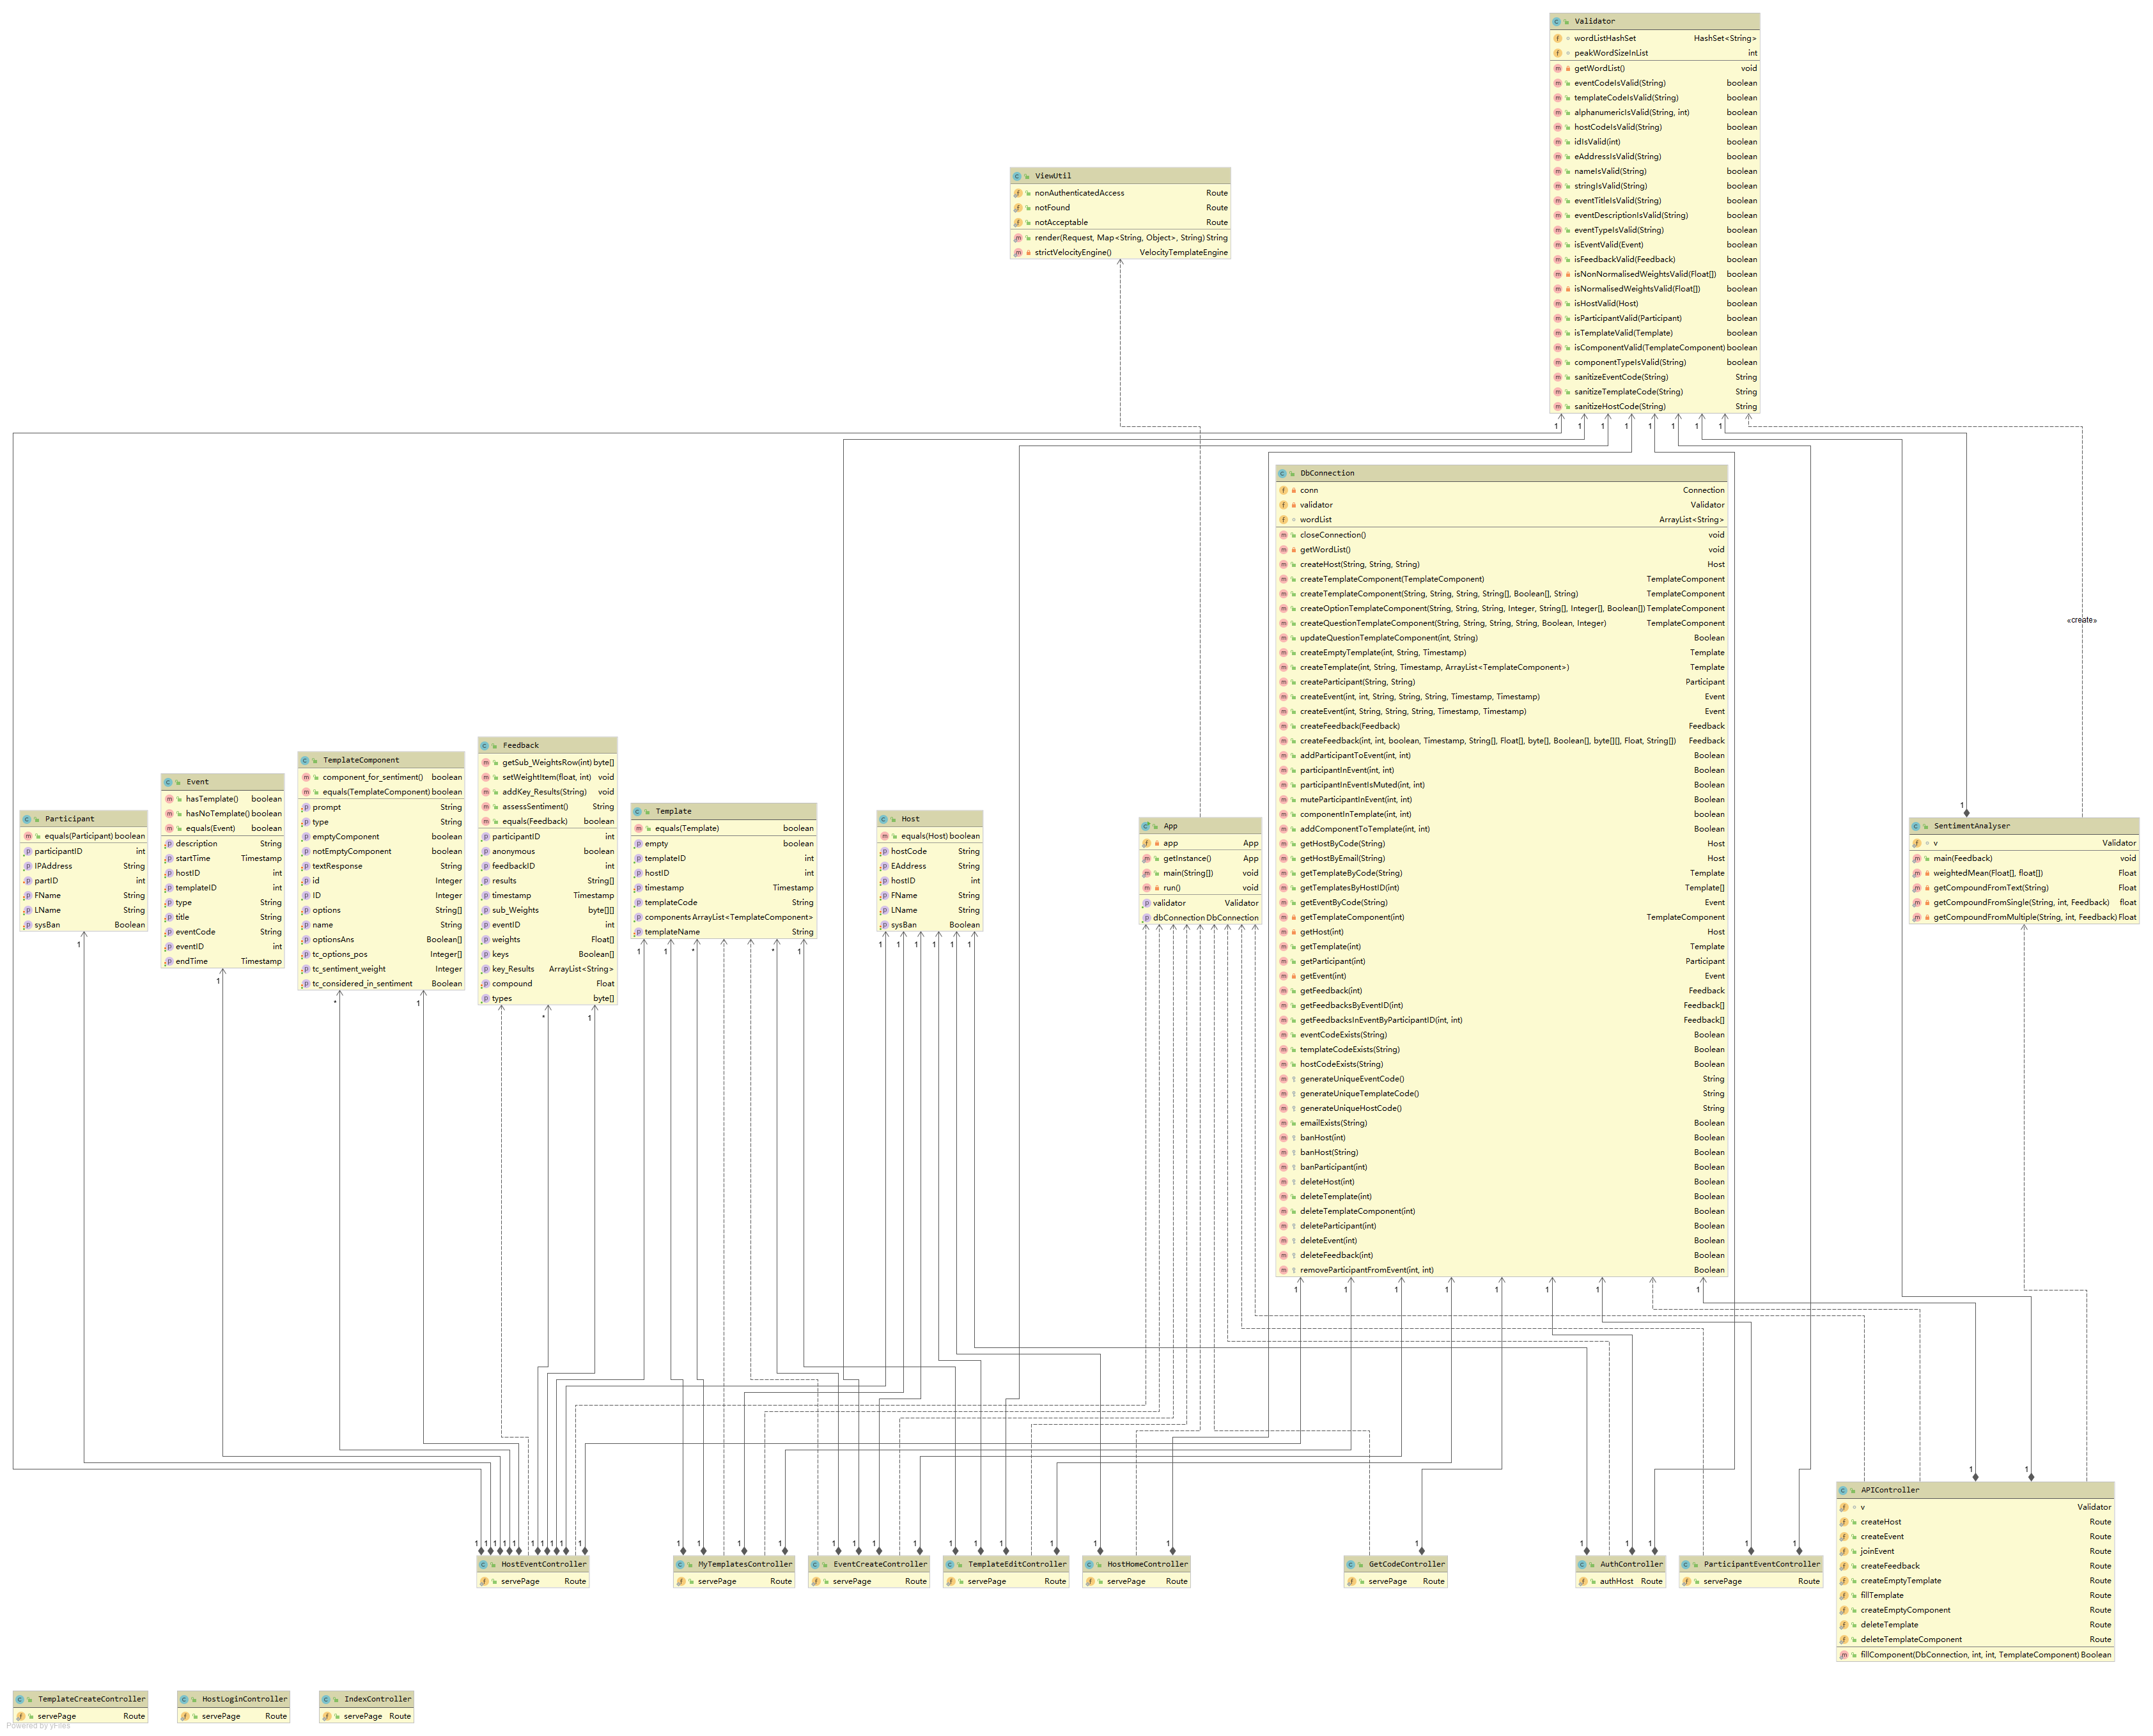
\includegraphics[height=7in,angle=90]{images/uml.png}
    \caption{A larger version of back-end UML class diagram; created with JetBrains IntelliJ IDEA.}
    \label{fig:uml-sideways}
\end{figure}

\end{document}